%\documentclass[a4paper,titlepage]{book}
\documentclass[a4paper,titlepage]{article}
\usepackage[utf8]{inputenc}
\usepackage[italian]{babel}

\usepackage{frontespizio}

\usepackage{subfig}
\usepackage{tikz}
\usepackage{listings}

\usepackage{booktabs}

%\usepackage{natbib}
\usepackage[style=alphabetic,backend=biber]{biblatex}
\addbibresource{reference.bib}
\usepackage{csquotes}

\usepackage{graphicx}
\usepackage{hyperref}

\usepackage{proof}


\title{La Modellazione di Protocolli di Sicurezza}
\author{Alessandro Busatto}
\date{\today}

\setcounter{secnumdepth}{2}


%grafica lstlisting
\lstdefinelanguage{XMI}{
  basicstyle=\ttfamily\footnotesize,
  keywordstyle=\color{blue}\bf,
  keywords={xmi,type, xmi, id, name, aggregation, classifier, packagedElement, /packagedElement, ownedComment, /ownedComment, ownedAttribute,  /ownedAttribute, body, /body, informationSource, informationTarget}
}

\lstdefinelanguage{app}{
  basicstyle=\ttfamily,
  keywordstyle=\it\bf,
  keywords={type, fun, reduc, free, forall, query, event, let, in, out}
}

\lstdefinelanguage{app_app}{
  basicstyle=\footnotesize,
  keywordstyle=\it\bf,
  keywords={type, fun, reduc, free, forall, query, event, let, in, out}
}


\lstdefinelanguage{vp}{
  basicstyle=\ttfamily,
  keywordstyle=\it\bf,
  keywords={attacker, principal, confidentiality,leaks, queries, authentication, knows, generates}
}


%\renewcommand\thesection{\arabic{section}}


\begin{document}

\maketitle

% \clearpage
% Scaletta originale del punto 2
% \bigskip
% 2. La Modellazione di Protocolli di Sicurezza:\\
% 	a. UML\\
% 		•  Object diagram e sequence diagram (pro e contro nell'utilizzo per la modellazione di protocolli e perchè nel nostro caso possiamo considerarli equivalenti)\\
% 	b. Collegamento del significato della rappresentazione dei blocchi UML (in particolare delle funzioni)\\
% 		•  Primitive cosa sono\\
% 		•  "Primitive" di encryption e decryption, come potrebbero essere rappresentate attraverso altre primitive e perchè con la semantica utilizzata vengono definite "primitive" (enc/dec vs concat/deconcat)\\
% 		•  Spiegazione dello stato dell'arte e del motivo per cui per la verifica formale dei protocolli si è scelto di utilizzare il modello di attaccante Dolev Yao rispetto all'obiettivo di trovare falle nei protocolli a prescindere dal tipo di attaccante\\
% 	c. Domain Specific Languages\\
% 		•  VerifPal lang, ProVerif lang etc.\\
% 	d. Il modello di Attaccante Dolev-Yao\\
	
% \clearpage

%\begin{minipage}{\textwidth}
%    \vfill
\tableofcontents
\listoffigures
\thispagestyle{empty}
%\end{minipage}
\clearpage

\setcounter{page}{1}
\section{Modellazione dei protocolli mediante UML}

Per la modellazione di protocolli\footnote{per protocolli si intendono protocolli di sicurezza come Needham Schroeder Symmetric Key, protocolli di comunicazione come ARP e protocolli di encryption come RSA} si è deciso di utilizzare lo standard UML (Unified Modeling Language) nella versione 2.4\footnote{\url{https://www.omg.org/spec/UML/2.4/About-UML/}}, perch\'e questo tipo di modellazione utilizza una notazione semi-grafica che consente al progettista di ragionare sulla logica del protocollo che \`e pi\`u semplice rispetto al codice, senza dover porre eccessiva attenzione a come effettivamente deve essere implementato e senza dover necessariamente scrivere codice per la sua rappresentazione.\\  
Esistono 14 tipi di diagrammi nella modellazione UML, suddivisi in diagrammi strutturali e diagrammi comportamentali (o di interazione).\\ 
Tra i vari tipi di diagrammi troviamo il sequence diagram, un diagramma comportamentale, definito per la rappresentazione dettagliata delle interazioni tra gli agenti (componenti hardware o software) partecipanti al protocollo, per sua natura risulta essere il diagramma più adatto alla rappresentazione dei protocolli.\\ 
Una caratteristica di questo tipo di diagramma è che l'asse verticale rappresenta il tempo, quindi è possibile rappresentare l'ordine cronologico delle interazioni tra gli agenti partecipanti, dall'alto verso il basso.\\
In alternativa può essere utilizzato l'object diagram, un diagramma di tipo strutturale nel quale vengono rappresentate le relazioni tra i vari oggetti che compongono il sistema, nel nostro caso le relazioni e gli oggetti corrispondono rispettivamente a interazioni e agenti del sequence diagram.\\
Gli altri 12 tipi di diagramma sono stati esclusi dai possibili diagrammi utili per rappresentare protocolli perch\'e descrivono aspetti ortogonali alle interazioni descritte nel sequence diagram.\\
Nella Sezione \ref{sub:con} verrà spiegato in dettaglio perch\'e si può utilizzare indifferentemente uno tra il sequence diagram e l'object diagram.

\subsection{Confronto tra sequence diagram e object diagram}\label{sub:con}

Per la modellazione tramite lo standard UML è stato utilizzato il tool, open source, Modelio\footnote{\url{https://www.modelio.org/}} nella versione 4.1.\\
Dato il protocollo Needham Schroeder Symmetric Key descritto in \cite{NS78}:
\begin{lstlisting}[mathescape]
    1. $A \rightarrow S : A, B, N_a$
    2. $S \rightarrow A : \{N_a, K_{ab}, B, \{K_{ab}, A\}_{K_{bs}}\}_{K_{as}}$
    3. $A \rightarrow B : \{K_{ab}, A\}_{K_{bs}}$
    4. $B \rightarrow A : \{N_b\}_{K_{as}}$
    5. $A \rightarrow B : \{N_b-1\}_{K_{as}}$
\end{lstlisting}
\noindent Dove:
\begin{itemize}
    \item $X \rightarrow Y : m$ indica che il principal \texttt{X} invia un messaggio al principal \texttt{Y},
    \item $N_x$ indica il nonce generato dal principal \texttt{X},
    \item $K_{xy}$ indica la chiave condivisa tra i principal \texttt{X} e \texttt{Y},
    \item $\{\dots\}_{K_{xy}}$ indica che il pacchetto è cifrato con la chiave condivisa tra i principal \texttt{X} e \texttt{Y}.
\end{itemize}
Le figure \ref{fig:sd}-\ref{fig:od}, rappresentano il terzo messaggio del protocollo rispettivamente con un sequence ed un object diagram.\\
Più precisamente vengono rappresentate le operazioni fatte dall'agente \texttt{A} una volta ricevuta la chiave simmetrica da utilizzare con \texttt{B} dal server \texttt{S}.\\
L'agente \texttt{A} decifra con la chiave condivisa con il server \texttt{S} il pacchetto, ed inoltra all'agente \texttt{B} il pacchetto cifrato con la chiave condivisa tra \texttt{B} e \texttt{S}, contenente la chiave simmetrica tra \texttt{A} e \texttt{B}.\\

\begin{figure}[h!] 
    \centering 
        \includegraphics[width=0.8\textwidth]{../img/FirstMessage.png} 
        \caption{Sequence diagram: Inoltro pacchetto da \texttt{A} a \texttt{B}} 
        \label{fig:sd}
\end{figure}

\begin{figure}[h!]
    \centering 
    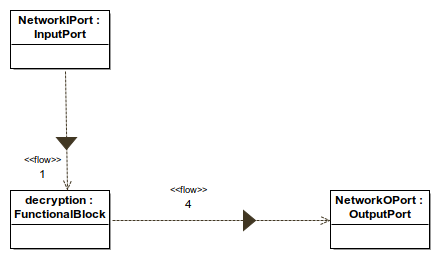
\includegraphics[scale=0.6]{../img/FirstMessage_2.png} 
    \caption{Object diagram: Inoltro pacchetto da \texttt{A} a \texttt{B}} 
    \label{fig:od}
\end{figure}

\begin{lstlisting}[frame=single, mathescape, basicstyle=\footnotesize]
1. $\{N_a, K_{ab}, B, \{K_{ab}, A\}_{K_{bs}}\}_{K_{as}}$
2. $\{N_a, K_{ab}, B, \{K_{ab}, A\}_{K_{bs}}\}_{K_{as}}$
3. $\{N_a, K_{ab}, B, \{K_{ab}, A\}_{K_{bs}}\}$
4. $\{K_{ab},A\}_{K_{bs}}$
\end{lstlisting}

\noindent Durante la fase di ingegnerizzazione di un sistema viene modellata la parte fisica, ovvero le componenti hardware che compongono il sistema, l'obiettivo è quello di unirla alla modellazione logica del funzionamento del protocollo attraverso la modellazione UML.\\
Per fare questo si è resa necessaria l'introduzione di nuovi tipi\footnote{con abuso di notazione, quando si parla di tipi di elementi, si intende la tipologia degli oggetti della classe istanziata} di elementi, che non appartengono ai tipi degli elementi standard dei diagrammi UML.\\
\begin{figure}[h!]
    \centering
    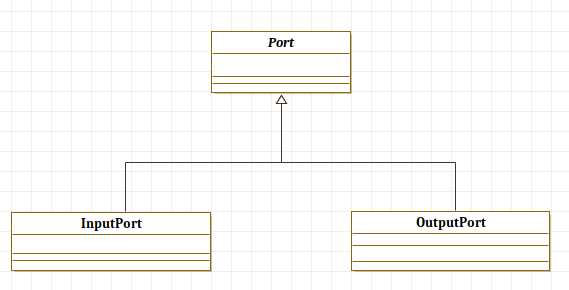
\includegraphics[width=0.6\textwidth]{../img/cdport.png} 
    \caption{Class diagram Port}
    \label{fig:cdport}
\end{figure}

\noindent Come vediamo in Figura \ref{fig:cdport} sono stati definiti i tipi InputPort e OutPort, specializzazioni del tipo Port.\\
Questi tipi di oggetti vengono utilizzati nelle due tipologie di diagramma come unico punto di contatto tra i modelli del software e dell'hardware, infatti sono le componenti utilizzate dai protocolli per ricevere o inoltrare messaggi.\\
Inoltre, guardando le lifelines in Figura \ref{fig:sd} si può notare anche il Controller, il quale è il dispositivo proprietario delle porte.\\
Anche per la modellazione logica del funzionamento del protocollo si è resa necessaria l'introduzione di nuovi tipi.\\
\begin{figure}[h!]
    \centering
    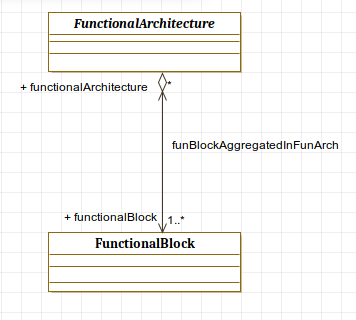
\includegraphics[width=0.5\textwidth]{../img/cdfun.png} 
    \caption{Class diagram Function}
    \label{fig:cdfun}
\end{figure}

\noindent Gli elementi di tipo FunctionalBlock vengono utilizzati per la codifica di un'operazione che non può essere dettagliata maggiormente (oppure non è necessario farlo considerando l'obiettivo della verifica di questo modello) che, presi degli input, restituisce un output.\\
Nel caso in cui si voglia rappresentare un insieme di operazioni si utilizzano gli elementi di tipo FunctionalArchitecture, questi vengono utilizzati come ``segnaposto'' per l'insieme di operazioni che verrà descritto in un altro diagramma dello stesso tipo di quello utilizzato, avente come nome lo stesso dato all'elemento di tipo FunctionalArchitecture.\\
Infatti come vediamo in Figura \ref{fig:cdfun} una FunctionalArchitecture può essere composta da uno o più elementi di tipo FunctionalBlock.\\
In entrambi i diagrammi le InformationFlow rappresentano gli input e gli output dei vari elementi, nelle etichette vengono descritti i parametri passati, per convenzione se i parametri si trovano tra \{ \} significa che l'input o l'output di un oggetto è un pacchetto.\\
Modelio consente di esportare i modelli UML in file .xmi (XML Metadata Interchange), uno standard basato sulla struttura XML che ne consente lo scambio tra applicazioni.\\
Nel file .xmi, strutturato come un xml, troviamo i tag per l'identificazione tramite codice univoco (id) degli elementi (lifelines, oggetti, InformationFlow) e i tag per descrivere le proprietà dei vari elementi (tipo, nome, descrizione). Tra le proprietà degli elementi di tipo InformationFlow sono presenti i tag per identificare tramite id l'elemento sorgente e l'elemento destinazione delle informazioni. Analizzando il file .xmi estratto da un protocollo modellato tramite sequence diagram (Listing \ref{fig:sdxmi}) o da un protocollo modellato tramite object diagram (Listing \ref{fig:odxmi}), possiamo vedere come l'estrazione delle lifelines del sequence diagram corrisponde all'estrazione degli oggetti dell'object diagram (righe 7-12) e l'estrazione delle information flow viene rappresentata nello stesso modo (righe 14-20).\\
\begin{minipage}{0.48\textwidth}
      \centering
      \lstinputlisting[label={fig:sdxmi},caption={Estratto di XMI da sequence diagram},mathescape,numbers=left, language=XMI, breaklines= true, frame=single]{../xmi/ns_estratto_seq_2.xmi}
    \end{minipage}\hfill
    \begin{minipage}{0.48\textwidth}
      \centering
      \lstinputlisting[label={fig:odxmi},caption={Estratto di XMI da object diagram},mathescape, language=XMI, breaklines= true, frame=single]{../xmi/ns_estratto_ob_2.xmi} 
\end{minipage}
\newpage

\noindent Questo ci consente di affermare che utilizzando uno a scelta tra i due diagrammi è possibile modellare un protocollo senza la perdita di alcuna informazione.\\
Il file .xmi può essere utilizzato come input di un software in grado di navigarne la struttura e restituire in output dei file pronti per essere utilizzati dai tool di verifica formale e automatica dei protocolli, ad esempio nella Sezione \ref{sez:tc} viene presentato un software, da me sviluppato, in grado di restituire come output un file scritto nel linguaggio specifico per essere utilizzato come input dal tool di verifica automatica VerifPal.

\begin{figure}[h!]
    \centering
    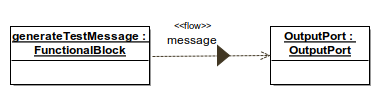
\includegraphics[scale=0.6]{../xmi/ex.png} 
    \caption{Esempio di modellazione con object diagram}
    \label{fig:exUML}
\end{figure}

\begin{figure} [h!]
    \centering
    \lstinputlisting[language=XMI, breaklines= true, frame=single]{../xmi/ex.xmi}
    \caption{Esempio di estrazione di un file .xmi}
\end{figure}

\clearpage

\clearpage
\newpage
\subsection{Modellazione di protocolli con UML}
%\fixnote{mr}{non possiamo avere cos\`i tanti esempi senza spiegazione. O li raccontiamo o li togliamo. Se ``spaccano'' troppo il testo possiamo spostarli in appendice. Inoltre le immagini sono difficili da leggere perch\'e ci sono troppi a-capo nei blocchi. Inoltre le varie immagini sono zoomate diversamente, io renderei pi\`u omogeneo.}
\subsubsection*{Needham Schroeder Symmetric Key}
In questa sezione vedremo come è possibile modellare attraverso i diagrammi object diagram dello standard UML il protocollo di sicurezza a chiave simmetrica proposto da Needham e Schroeder:
\begin{lstlisting}[mathescape]
    1. $A \rightarrow S : A, B, N_a$
    2. $S \rightarrow A : \{N_a, K_{ab}, B, \{K_{ab}, A\}_{K_{bs}}\}_{K_{as}}$
    3. $A \rightarrow B : \{K_{ab}, A\}_{K_{bs}}$
    4. $B \rightarrow A : \{N_b\}_{K_{as}}$
    5. $A \rightarrow B : \{N_b-1\}_{K_{as}}$
\end{lstlisting} 

\noindent Nelle Figure seguenti avremo i seguenti partecipanti al protocollo: l'agente Initiator che vuole iniziare la comunicazione con l'agente Recipient e richiede la password per la comunicazione al server S.\\
Inoltre la chiave simmetrica viene rappresentata in questo modo SK(a,b), dove a e b indicano l'identità degli agenti proprietari della chiave.\\

\begin{figure}[h!] 
    \centering 
    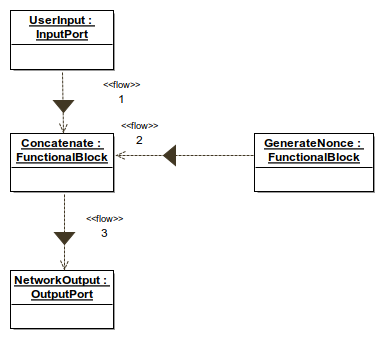
\includegraphics[scale=0.6]{img/NSSK/First_message(toServer)_Object diagram.png} 
    %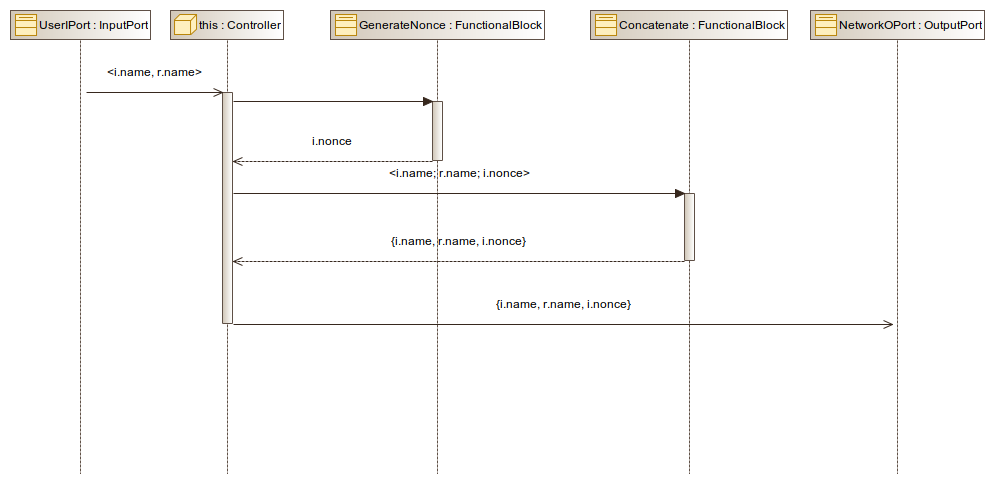
\includegraphics[width=\textwidth]{img/NSSK/Sequencediagram/First_Message(toServer).png} 
    \begin{lstlisting}[frame=single, mathescape, basicstyle=\footnotesize]
        1. $<i.name, r.name>$
        2. $<i.nonce>$
        3. $<i.name, r.name, i.nonce>$
    \end{lstlisting}
    \caption{$A \rightarrow B : A, B, N_a$} 
\end{figure}
\noindent Nell'oggetto UserInput il sistema che andrà ad implementare il protocollo riceve il nome ($r.name$) dell'agente Recipient, l'oggetto GenerateNonce genera un nuovo Nonce e l'oggetto Concatenate prepare il pacchetto, da mandare al server S attaverso l'oggetto NetworkOPort, composto da $i.name, r.name, i.nonce$, ovvero dai nomi dei partecipanti al protocollo e il nonce per assicurarsi che la comunicazione sia fresh.
\newpage
\begin{figure}[h!] 
    \centering 
    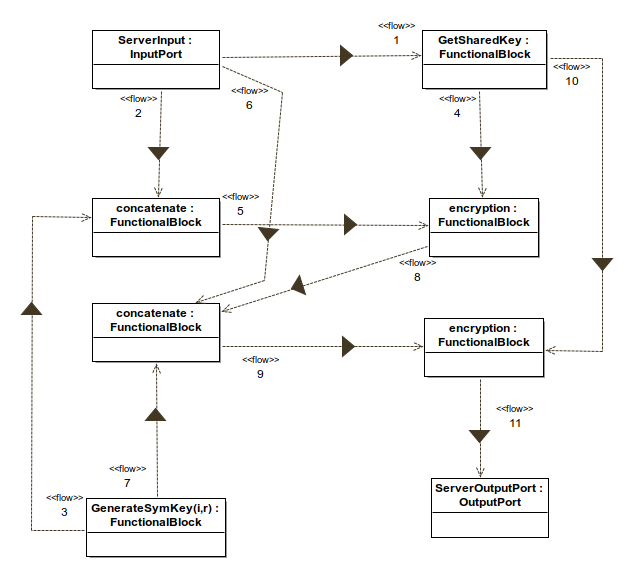
\includegraphics[scale=0.5]{img/NSSK/Second_Message(fromServer).png} 
    %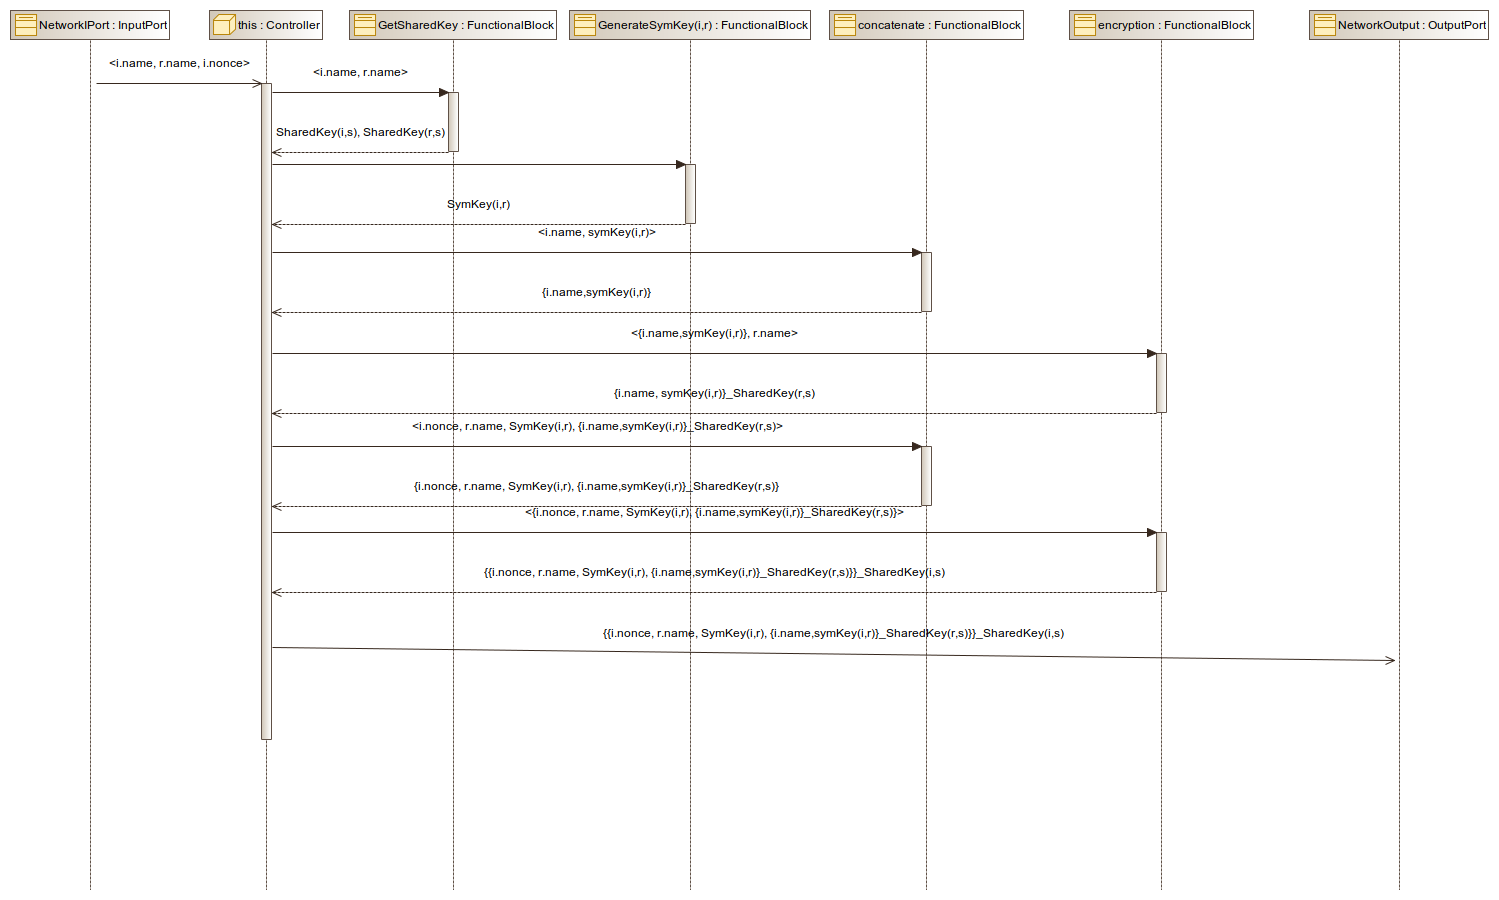
\includegraphics[width=\textwidth]{img/NSSK/Sequencediagram/Second_Message(fromServer).png} 
    \begin{lstlisting}[frame=single, mathescape, basicstyle=\footnotesize]
        1. $<i.name,r.name>$
        2. $<i.name>$
        3. $<SK(i,r)>$
        4. $<SK(s,r)>$
        5. $<i.name, SK(i,r)>$
        6. $<r.name, i.nonce>$
        7. $<SK(i,r)>$
        8. $<\{i.name; SK(i,r)\}\_SK(r,s)>$
        9. $<i.nonce, r.name, SK(i,r), \{i.name,SymKey(i,r)\}\_SK(r,s)\}>$
        10. $<SK(s,r)>$
        11. $<\{i.nonce, r.name, SK(i,r), \{i.name,SK(i,r)\}\_SK(rs)\}\}\_SK(i,s)>$
    \end{lstlisting}
    \caption{$S \rightarrow A : \{N_a, K_{ab}, B, \{K_{ab}, A\}_{K_{bs}}\}_{K_{as}}$} 
\end{figure}
\noindent Una volta ricevuto il pacchetto, il server S provvede alla generazione della chiave simmetrica (SK(i,r)) per la comunicazione tra Initiator e Recipient utilizzando l'oggetto GenerateSymKey(i,r), passando a quest'ultimo i nomi $i.name, r.name$ dei partecipanti.\\ 
A questo punto, fornendo sempre come input i nomi dei partecipanti all'oggetto GetSharedKey, ottiene le chiavi simmetriche precedentemente condivise tra lui e ogni agente partecipante (SK(i,s) e SK(r,s)).\\ 
La chiave SK(r,s) verrà utilizzata dall'oggetto encryption dopo aver preparato con l'oggetto Concatenate il pacchetto per l'agente Recipient, questo pacchetto a sua volta verrà inserito da un altro oggetto Concatenate nel pacchetto per l'agente Initiator e il tutto verrà cifrato da un'altro oggetto encryption con la chiave SK(i,s). Il pacchetto risultante da queste operazioni verrà spedito all'agente Initiator attraverso l'oggetto ServerOutputPort.\\

\begin{figure}[h!] 
    \centering 
    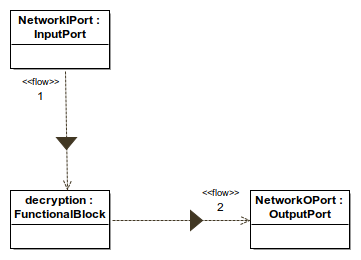
\includegraphics[scale=0.6]{img/NSSK/FirstMessage.png} 
    %\includegraphics[width=\textwidth]{img/NSSK/Sequencediagram/FirstMessage.png}
    \begin{lstlisting}[frame=single, mathescape, basicstyle=\footnotesize]
        1. $<\{i.nonce, r.name, SK(i,r), \{i.name,SK(i,r)\}\_SK(r,s)\}\_SK(i,s)>$
        2. $<\{i.name,SK(i,r)\}\_SK(r,s)>$
    \end{lstlisting}
    \caption{$A \rightarrow B : \{K_{ab}, A\}_{K_{bs}}$} 
\end{figure}
\noindent L'agente Initiator riceve il pacchetto attraverso l'oggetto NetworkIPort e utilizza l'oggetto di decryption con la chiave simmetrica SK(i,s) per estrarre il pacchetto da inoltrare all'agente Recipient attraverso l'oggetto NetworkOPort.\\
\begin{figure}[h!] 
    \centering 
    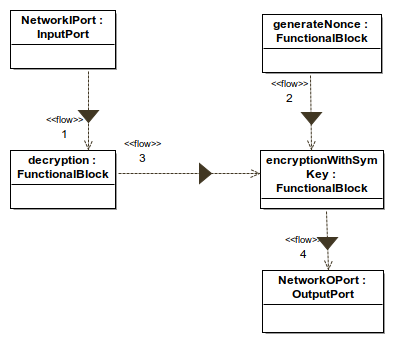
\includegraphics[scale=0.59]{img/NSSK/SecondMessage.png} 
    %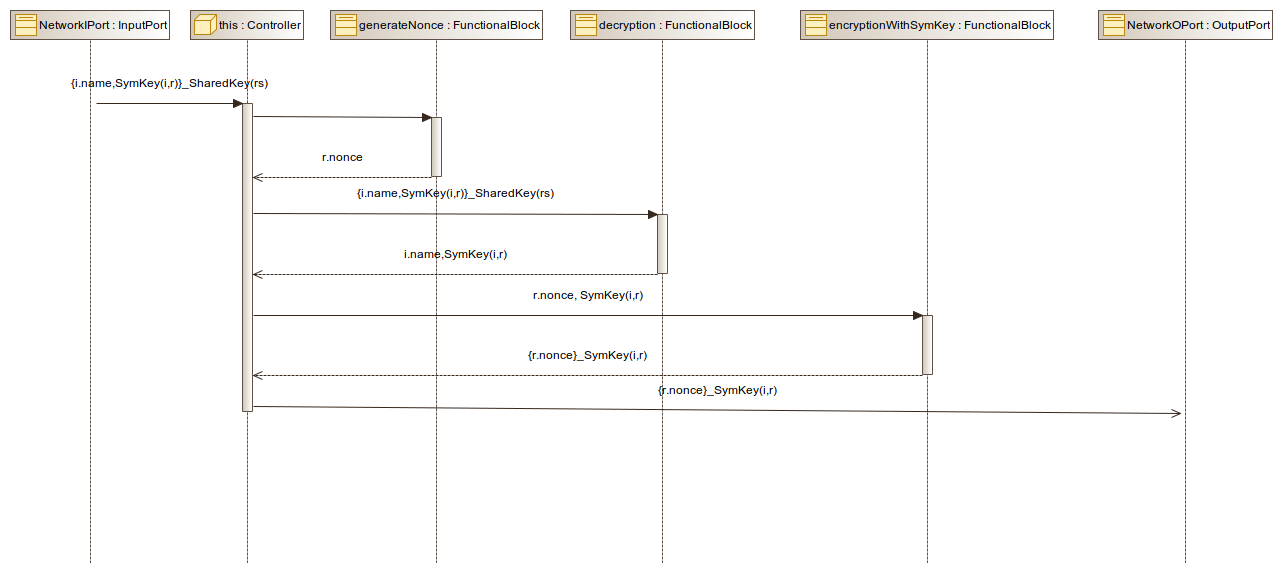
\includegraphics[width=\textwidth]{img/NSSK/Sequencediagram/SecondMessage.png} 
    \begin{lstlisting}[frame=single, mathescape, basicstyle=\footnotesize]
        1. $<\{i.name,SK(i,r)\}\_SK(r,s)>$
        2. $<r.nonce>$
        3. $<SK(i,s)>$
        4. $<\{r.nonce\}\_SK(i,r)>$
    \end{lstlisting}
    \caption{$B \rightarrow A : \{N_b\}_{K_{as}}$} 
\end{figure}
\newpage
\noindent L'agente Recipient riceve il pacchetto attraverso l'oggetto NetworkIPort, lo decifra con l'oggetto decryption utilizzando la chiave SK(r,s) ed estrae la chiave SK(i,r).\\ 
SK(i,r) verrà utilizzata dall'oggetto encryptionWithSymKey per cifrare un nuovo pacchetto contenente il Nonce generato dall'oggetto generateNonce.\\ 
Infine l'agente Recipient spedisce il pacchetto all'agente Initiator utilizzando l'oggetto NetworkOPort.\\
\begin{figure}[h!] 
    \centering 
    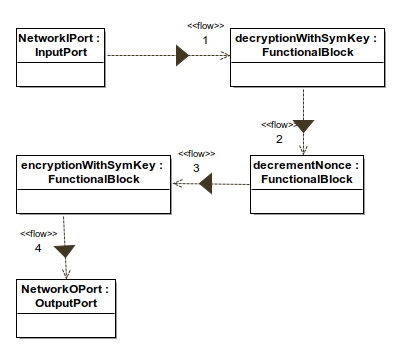
\includegraphics[scale=0.6]{img/NSSK/ThirdMessage.png} 
    %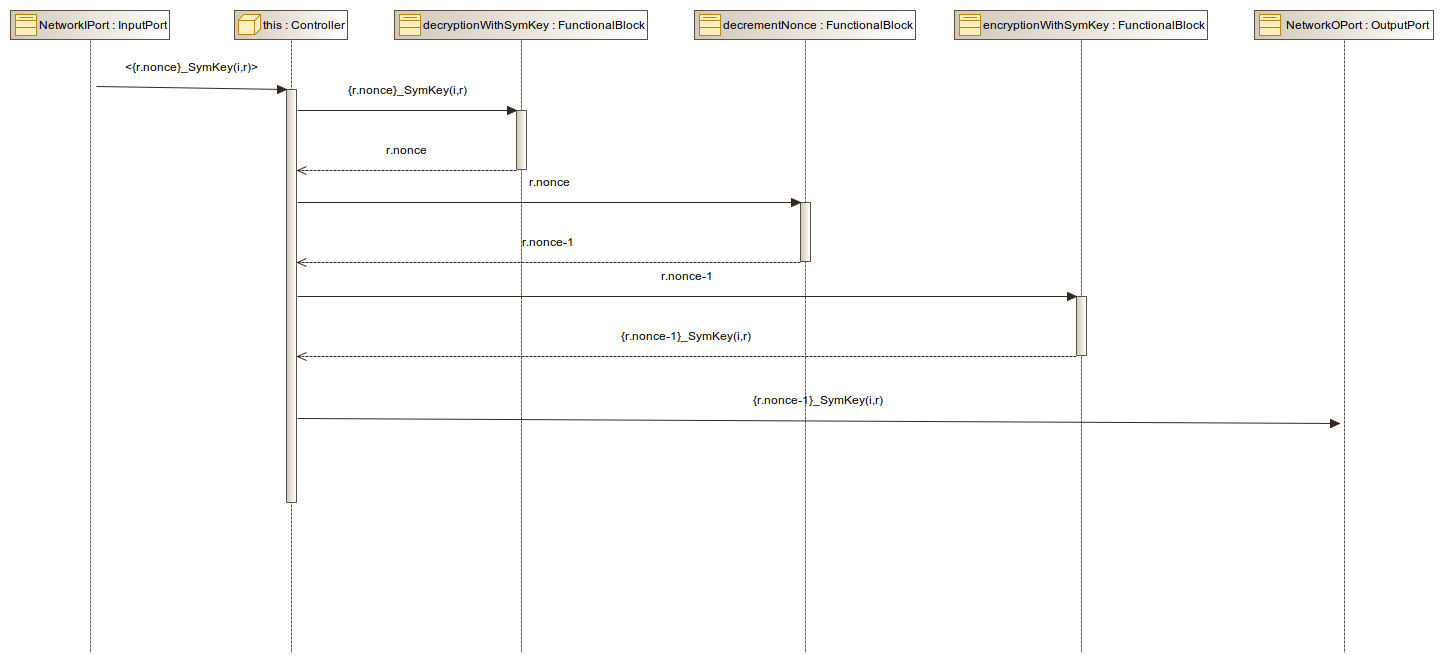
\includegraphics[width=\textwidth]{img/NSSK/Sequencediagram/ThirdMessage.png} 
    \begin{lstlisting}[frame=single, mathescape, basicstyle=\footnotesize]
        1. $<{r.nonce}\_SK(i,r)>$
        2. $<r.nonce>$
        3. $<r.nonce-1>$
        4. $<\{r.nonce-1\}\_SK(i,r)>$
    \end{lstlisting}
    \caption{$A \rightarrow B : \{N_b-1\}_{K_{as}}$} 
\end{figure}\\
\noindent Nell'ultima fase del protocollo, l'agente Initiator riceve dall'oggetto NetworkIPort il pacchetto contenente il Nonce, lo decifra con l'oggetto decryptionWithSymKey utilizzando la chiave SK(i,r), utilizza l'oggetto decrementNonce per sottrarre 1 al Nonce inviato dall'agente Recipient e cifra il risultato con l'oggetto encryptionWithSymKey utilizzando la chiave SK(i,r).\\
Il pacchetto risultante viene spedito all'agente Recipient attraverso l'oggetto NetworkOPort.\\

\newpage
\subsubsection*{Address Resolution Protocol}
Lo scopo del protocollo ARP descritto in \cite{RFC0826} e in \cite{RFC5227} è quello di eseguire una mappatura tra indirizzo IP e indirizzo MAC di una macchina all'interno di una rete locale Ethernet.\\
La notazione seguente utilizzata nei pacchetti è ripresa da \cite{RFC0826}:
\begin{lstlisting}
    ar$hrd: Hardware address space 
    ar$pro: Protocol address space
    ar$hln: byte length of each hardware address
    ar$pln: byte length of each protocol address
    ar$op:  opcode (request | reply)
    ar$sha: Hardware address of sender 
    ar$spa: Protocol address of sender 
    ar$tha: Hardware address of target
    ar$tpa: Protocol address of target
\end{lstlisting}
In Figura \ref*{fig:ARP} vediamo come si modella il protocollo ARP.\\
Una macchina, appena connessa alla rete o accesa, si mette subito in ascolto con l'oggetto ANNUNCE\_AWAIT e, allo stesso tempo, utilizza gli oggetti getIPAddress per generare un indirizzo IP sul quale essere contattata, getProtocolType e getMACAddress  per ricavare informazioni sul tipo di protocollo ethernet da utilizzare e l'indirizzo MAC della sua scheda di rete.\\
A questo punto utilizza queste informazioni per creare attraverso l'oggetto createProbePackage un pacchetto da inviare in broadcast a tutte le macchine della rete.\\
Successivamente attende un tempo predefinito attraverso l'oggetto PROBE\_WAIT, prima di spedire il pacchetto attraverso l'oggetto EthernetOUT e ritornare nello stato di ANNUNCE\_WAIT.\\
Se nell'arco di un tempo predefinito non arriva nessun pacchetto dall'oggetto EthernetIN, procede con la conferma dell'indirizzo IP attraverso la creazione di un nuovo pacchetto con l'oggetto createAnnuncePackage, il quale verra sempre spedito in broadcast attraverso l'oggetto EthernetOUT.\\
Se invece riceve un pacchetto dall'oggetto EthernetIN, ricomincia generando un nuovo indirizzo IP.\\
\newpage
\begin{figure}[h!] 
    \centering 
    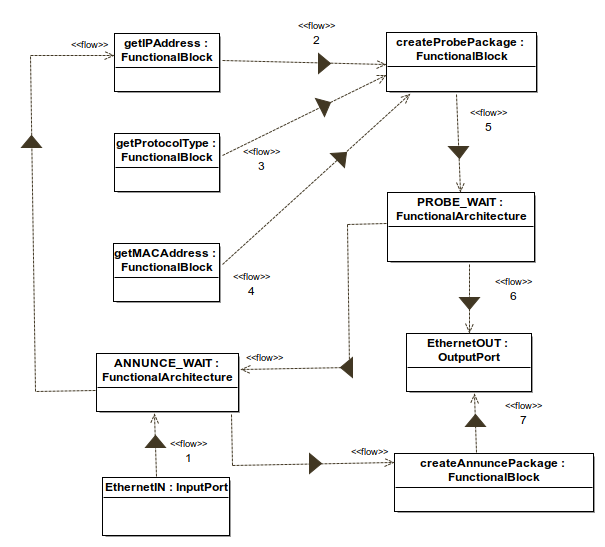
\includegraphics[scale=0.6]{img/ARP/ARP.png} 
    \begin{lstlisting}[frame=single, mathescape, basicstyle=\footnotesize]
1. $<\{as\$hrd, ar\$pro, ar\$hln, ar\$pln, reply, ar\$sha, ar\$spa, ar\$tha, ar\$tpa\}>$
2. $<ip>$
3. $<ar\$spa>$
4. $<ar\$sha>$
5. $<\{as\$hrd, ar\$pro, ar\$hln, ar\$pln, request, ar\$sha, 0.0.0.0, 00:00:00:00:00:00, ip\}>$
6. $<\{as\$hrd, ar\$pro, ar\$hln, ar\$pln, request, ar\$sha, 0.0.0.0, 00:00:00:00:00:00, ip\}>$
7. $<\{as\$hrd, ar\$pro, ar\$hln, ar\$pln, request, ar\$sha, ip, 00:00:00:00:00:00, ip\}>$
    \end{lstlisting}
    \caption{Modellazione del protocollo ARP} 
    \label{fig:ARP}
\end{figure}
\newpage
\begin{figure}[h!] 
    \centering 
    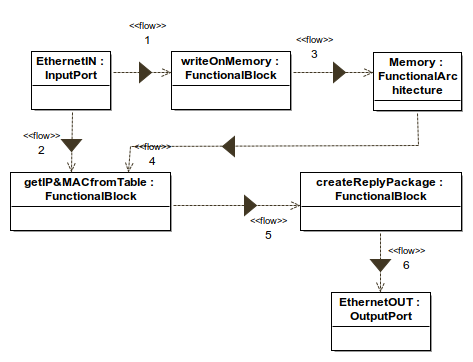
\includegraphics[scale=0.6]{img/ARP/ARP_Reply_Object_diagram.png} 
\begin{lstlisting}[frame=single, mathescape, basicstyle=\footnotesize]
1. $<\{as\$hrd, ar\$pro, ar\$hln, ar\$pln, request, ar\$sha, ip, 00:00:00:00:00:00, ip\}>$
2. $<\{as\$hrd, ar\$pro, ar\$hln, ar\$pln, request, ar\$sha, 0.0.0.0, 00:00:00:00:00:00, ip\}>$
3. $<ar\$sha, ip>$
4. $<ar\$tha, ar\$tpa>$
5. $<ar\$tha, ar\$tpa>$
6. $<\{as\$hrd, ar\$pro, ar\$hln, ar\$pln, reply, ar\$sha, ar\$spa, ar\$tha, ar\$tpa\}>$
\end{lstlisting}
    \caption{Modellazione del blocco di ARP Reply} 
\end{figure}
\noindent Nel caso in cui una macchina della rete riceva un pacchetto dall'oggetto EthernetIN, la prima cosa che fa è verificare se si tratta di un pacchetto di probe oppure di un pacchetto di annunce.\\
Nel primo caso va a verificare con l'oggetto Memory se nell'ARP cache è già presente quell'indirizzo IP, assegnato ad un indirizzo MAC, che non corrisponde a quello del sender del pacchetto.\\ 
Se vi è una corrispondenza tra l'indirizzo ip del sender del pacchetto ed uno già presente nell'ARP cache, allora l'oggetto getIP\&MACFromTable riceve in input le informazioni dalla ARP cache per generare un nuovo pacchetto attraverso l'oggetto createReplyPackage, con il quale rispondere in unicast al sender attraverso l'oggetto EthernetOut, altrimenti non fa nulla.\\
Nel caso in cui si tratti di un pacchetto di annunce allora l'oggetto writeOnMemory si occuperà di salvare nella ARP cache la mappatura tra l'indirizzo IP e MAC del sender.\\
\newpage
\clearpage
\subsubsection*{RSA}
Nel 1978 in \cite{RSA78} Rivest, Shamir e Adleman hanno proposto un crittosistema per la cifratura e la firma dei messaggi basato sulla crittografia asimmetrica.\\
Come vedremo nelle Figure successive il crittosistema si basa su tre funzioni principali: funzione di generazione delle chiavi, funzione di encryption e funzione di decryption.\\
Nella modellazione UML ogni oggetto rappresenta le funzioni matematiche utilizzate dalle tre funzioni.\\ 
L'oggetto Memory viene utilizzato dalla funzione di generazione delle chiavi per salvare le informazioni riguardo la chiave pubblica e la chiave privata necessarie alle funzioni di encryption e decryption.\\  
\begin{figure}[h!] 
    \centering 
    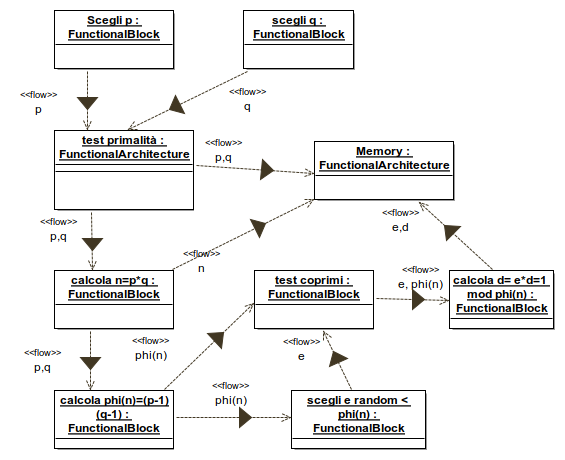
\includegraphics[scale=0.6]{img/RSA/Key_Generation_Object_diagram.png} 
    \caption{Generazione delle chiavi} 
\end{figure}
\begin{figure}[h!] 
    \centering 
    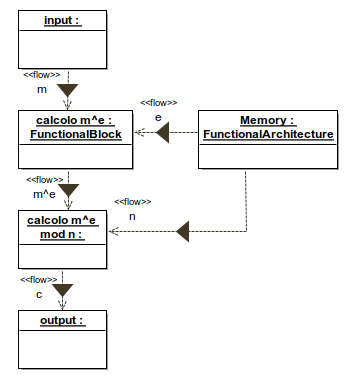
\includegraphics[scale=0.6]{img/RSA/Encryption_Object_diagram.png} 
    \caption{Funzione di encryption} 
\end{figure}
\newpage
\begin{figure}[h!] 
    \centering 
    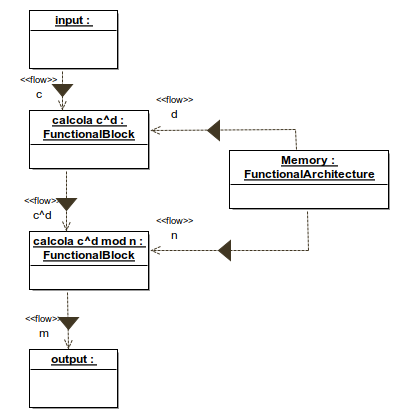
\includegraphics[scale=0.6]{img/RSA/Decryption_Object_diagram.png} 
    \caption{Funzione di decryption} 
\end{figure}
\newpage



    

\newpage
\section{Il modello di Attaccante Dolev-Yao}
\label{sec:dy}

In \cite{DY83}, gli autori hanno proposto un modello, noto anche come Dolev-Yao attacker model, per la formalizzazione degli attaccanti, questo modello viene comunemente utilizzato dai tool per la verifica formale dei protocolli basati sul modello simbolico, come vedremo con ProVerif e VerifPal.\\
Con questo tipo di modello si assume che l'attaccante sia in grado di:

\begin{itemize}
    \item intercettare, osservare ed eliminare i messaggi nella rete,
    \item costruire nuovi messaggi a partire da quelli osservati e iniettarli nella rete,
    \item disassemblare i messaggi non cifrati nelle parti che li compongono,
    \item iniettare nuovi messaggi nella rete costruiti con le informazioni di una sessione precendete del protocollo,
    \item decifrare messaggi cifrati solo se a conoscenza della chiave di cifratura.
\end{itemize}

\noindent L'attaccante di Dolev-Yao è un active attacker in grado di osservare, modificare ed eliminare i messaggi dalla rete, questo gli consente di utilizzare le regole descritte nella Figura \ref*{fig:rdy} per effettuare degli attacchi.\\
%L'attaccante Dolev-Yao è un attaccante che ha il pieno controllo della rete \fixnote{il DY \`e un active attacker}, può tentare ogni tipo di attacco possibile \fixnote{nope, pu\`o solo tentare quelli che gli vengono con le sue azioni.} grazie alla capacità di osservare, modificare ed eliminare i messaggi.\\
Nel modello Dolev-Yao si assume che la crittografia sia perfetta, ovvero che i meccanismi crittografici non siano vulnerabili, rendendo questo tipo di attaccante utile solo per attacchi alla logica dei protocolli.\\ 
%L'unica cosa che limita questo tipo di attaccante\fixnote{mr}{non userei limitato. Nel senso che il DY assume le primitive di encryption come blackbox, ma \`e anche limitato da tutte le azioni che non pu`\o fare. Per esempio, il social engineering non lo si pu\`o modellare, e nemmeno attacchi low level\ldots insomma credo sia buono per attacchi alla logica dei protocolli ma non di pi\`u} è l'assunzione della crittografia perfetta, ovvero l'assunzione per cui i meccanismi crittografici non sono vulnerabili, consentendo solo attacchi alla struttura del protocollo.\\
Grazie alle sue abilità, ai fini della verifica formale dei protocolli è utile identificare questo tipo di attaccante come la rete stessa.
%Questo tipo di attaccante è così potente\fixnote{non \`e una questione di potenza ma una scelta. Siccome ci fa comodo che l'attaccante venga identificato con la rete allora decidiamo che il DY lo sia. Questo rende l'attaccante molto forte} che è inutile differenziarlo dalla rete, si può dire che è la rete stessa.

\subsection{Primitive nel modello Dolev-Yao}
%\fix{mr}{forse \`e meglio citare il paper da cui hai preso il testo}
Considerando un attaccante attivo nel modello standard di Dolev e Yao, in grado di intercettare i messaggi, decifrarli solo se in possesso della chiave di decifratura, generarne di nuovi in base alla sua conoscenza e iniettarli nella rete immedesimando qualsiasi agente è possibile definire delle regole per il suo comportamento, come fatto in \cite{RVV17}. \\
Sia $\mathcal{S}$ un sistema e $\mathcal{S_{DY}}$ un sistema in presenza di attaccante del modello Dolev-Yao, sia IK un insieme di messaggi e DY(IK) il più piccolo insieme chiuso rispetto le regole del sistema  $\mathcal{S_{DY}}$ di generazione (G) e di analisi (A). \\
La regola G consente all'attaccante di generare nuovi messaggi a partire dai messaggi conosciuti, attraverso la concatenazione e utilizzando la crittografia simmetrica e asimmetrica, la regola A descrive come l'attaccante può decomporre i messaggi. 

\begin{figure}[h!]
    \centering
    \footnotesize
    \subfloat{\scalebox{0.85}{
    \begin{math}
    \infer[G_{assioma}]{M\in DY(IK)}{M\in IK}
    \end{math}
    }}
    \qquad
    \subfloat{\scalebox{0.85}{
    \begin{math}
        \infer[G_{concat}]{[M_1,M_2]\in DY(IK)}{M_1\in DY(IK) \quad M_2\in DY(IK)}
    \end{math}
    }}
    \\
    \subfloat{\scalebox{0.85}{
    \begin{math}
        \infer[G_{critA}]{\{M_1\}_{M_2}\in DY(IK)}{M_1\in DY(IK) \quad M_2\in DY(IK)}
    \end{math}
    }}
    \quad
    \subfloat{\scalebox{0.85}{
     \begin{math}
            \infer[G_{critS}]{\{|M_1|\}_{M_2}\in DY(IK)}{M_1\in DY(IK) \quad M_2\in DY(IK)}
    \end{math}
    }}
    \\
    \subfloat{\scalebox{0.85}{
    \begin{math}
        \infer[A_{concat_{i}}]{M_i\in DY(IK)}{[M_1,M_2]\in DY(IK)}
    \end{math}
    }}
    \quad
    \subfloat{\scalebox{0.85}{
    \begin{math}
        \infer[A_{critS}]{M_1\in DY(IK)}{\{|M_1|\}_{M_2}\in DY(IK) \quad M_2\in DY(IK)}
    \end{math}
    }}
    \\
    \subfloat{\scalebox{0.85}{
    \begin{math}
        \infer[A_{critA}]{M_1\in DY(IK)}{\{M_1\}_{M_2}\in DY(IK) \quad inv(M_2)\in DY(IK)}
    \end{math}
    }}
    \quad
    \subfloat{\scalebox{0.85}{
    \begin{math}
        \infer[A^{-1}_{critA}]{M_1\in DY(IK)}{\{M_1\}_{inv(M_2)}\in DY(IK) \quad M_2\in DY(IK)}
    \end{math}
    }}
    \caption{Sistema delle regole $\mathcal{S_{DY}}$ per l'attaccante Dolev-Yao}
    \label{fig:rdy}
\end{figure}

\newpage
\subsection{Le primitive nella modellazione UML}

Le primitive descritte nella Figura \ref{fig:rdy} vengono rappresentate anche nella modellazione del protocollo attraverso l'utilizzo dei diagrammi UML.\\
La primitiva $G_{concat}$ (concatenazione) appare nei diagrammi UML quando abbiamo più input in ingresso ad un oggetto con un singolo output, ad esempio viene utilizzata quando in un oggetto viene preparato un pacchetto, dati vari parametri in ingresso vengono concatenati prima di essere inoltrati.\\
Al contrario la primitiva $A_{concat}$ (deconcatenazione) appare quando abbiamo un singolo input e in uscita più output, come quando abbiamo in ingresso un pacchetto e dobbiamo ricavare qualche elemento da cui è composto.\\
\begin{figure}[h!] 
    \centering 
        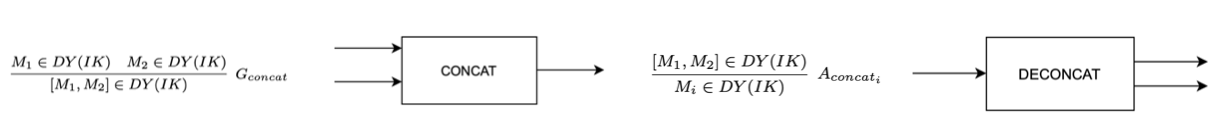
\includegraphics[width=\textwidth]{../img/1.png} 
        \caption{Concatenazione e deconcatenazione} 
\end{figure}\\
Nella modellazione UML gli oggetti di encryption e decryption sono considerati delle black box, questo perch\'e in caso di crittografia simmetrica corrispondono alle primitive $G_{critS}$ e $A_{critS}$ e in caso di crittografia asimmetrica corrispondono alle primitive $G_{crittA}$ e $A_{crittA}$ del modello Dolev-Yao.\\
\begin{figure}[h!] 
    \centering 
        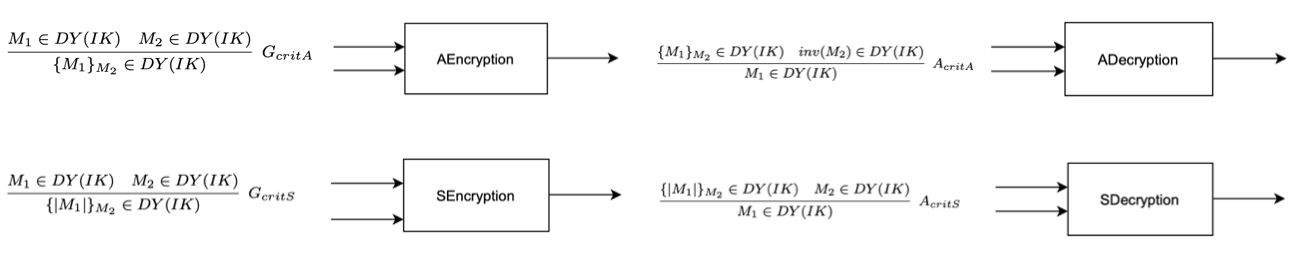
\includegraphics[width=\textwidth]{../img/2.png} 
        \caption{Encryption e decryption a chiave simmetrica e asimmetrica} 
\end{figure}\\
Nel caso in cui nel diagramma sia rappresentato un oggetto per la firma di un messaggio o per la verifica della firma, ancora una volta troviamo nel modello Dolev-Yao le primitive necessarie, ovvero la primitiva  $G_{crittA}$, la quale si occupa della firma di un messaggio prendendo come input la chiave privata e il messaggio, e la primitiva $A^{-1}_{crittA}$, la quale verifica la firma utilizzando la chiave pubblica.\\
\begin{figure}[h!] 
    \centering 
        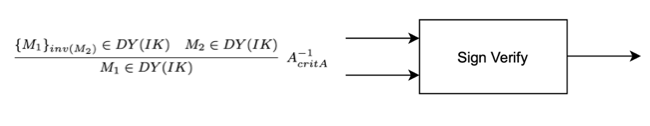
\includegraphics[width=0.6\textwidth]{../img/3.png} 
        \caption{Verifica della firma} 
\end{figure}\\
\begin{figure}[h!] 
    \centering 
        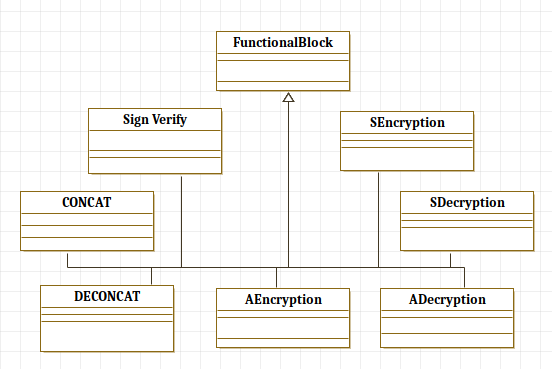
\includegraphics[width=0.8\textwidth]{../img/cd_1.png} 
        \caption{Diagramma delle classi delle primitive} 
\end{figure}\\





\newpage
\section{Analisi dello stato dell'arte}

La sicurezza delle informazioni viene definita utilizzando tre concetti di base:
confidenzialità, integrità e disponibilità, conosciuti anche con l'acronimo CIA (Confidentiality, Integrity e Availability).\\
Per confidenzialità si intende la proprietà che impedisce a individui, entità o processi non autorizzati di accedere alle informazioni, per integrità si intende la proprietà dei dati che ne vieta l'alterazione accidentale o eseguita da una terza parte malevola, comprendendo il caso limite di generazione ex novo di dati, infine per disponibilità si intende la capacità di accedere in qualsiasi momento ai dati richiesti.\\
Il solo utilizzo di queste tre proprietà è stato spesso criticato perch\'e ritenuto troppo generale per essere effettivamente applicato durante l'ingegnerizzazione di sistemi.\\
Per questo motivo molti ricercatori e organizzazioni hanno cercato di estendere la CIA con altre proprietà, ad esempio con l'autenticazione utilizzata proprio nelle proprietà di confidenzialità e integrità.\\
L'estensione della CIA negli anni è documentata nell'articolo \cite*{SC14} ed è riassunta nella Tabella \ref{tab:cia}.

\begin{table}[h!]
    \begin{tabular}{@{}lll@{}}
    \toprule
    \textbf{Anni} & \textbf{Definizione} & \textbf{Legenda}                                          \\ \midrule
    1970         & infosec = CIA        & Confidenzialità, Integrità, Disponibilità                 \\
    1980         & infosec += (Au,nR)   & Autenticazione e non-Ripudio                              \\
    1990         & infosec += CSpec     & Correttezza delle specifiche                              \\
    2000         & infosec += RITE      & Responsabilità, Integrità delle persone, fiducia, \\ 
    & & eticità\\
    \bottomrule
    \end{tabular}
    \caption{Evoluzione della CIA}
    \label{tab:cia}
    \end{table}

\noindent Per raggiungere obiettivi di sicurezza, come confidenzialità o autenticazione dei dati nella rete, anche in presenza di attaccanti, si sono sviluppati i protocolli di sicurezza, questi ultimi descrivono come gli agenti si scambiano messaggi utilizzando le primitive crittografiche.\\
Effettuare dei test di sicurezza è complesso, soprattutto quando si devono testare dei protocolli, per questo motivo l'utilizzo di tool automatici per la verifica può essere utile per ottenere garanzie sulla correttezza dei protocolli di sicurezza.\\
Grazie agli sforzi della ricerca per trovare nuovi protocolli sempre più sicuri, al giorno d'oggi è possibile trovarli implementati nella maggior parte delle applicazioni commerciali.\\ 
Sin dal 1976 con la ricerca di Diffie-Hellman si è cercato un modo per dimostrare che un protocollo soddisfacesse determinate proprietà di sicurezza, per fare questo dalla ricerca di Dolev-Yao nel 1983 sono nate due tecniche per testare la correttezza dei protocolli.\\
La prima tecnica è conosciuta come modello computazionale (o crittografico), mentre la seconda tecnica è conosciuta come modello simbolico (o metodo formale).\\
Queste due tecniche si basano sulla matematica formale per l'esecuzione di protocolli in ambienti con la presenza di uno o più attaccanti, l'obiettivo è quello di definire formalmente le proprietà di sicurezza previste dal sistema crittografico e sviluppare metodi per dimostrare rigorosamente la soddisfazione delle stesse.\\
Le caratteristiche principali del modello computazionale sono i modelli per l'esecuzione del sistema dettagliati a livello di bit e l'utilizzo di un attaccante potente, la sicurezza viene valutata rispetto a macchine probabilistiche a tempo polinomiale e questo fa si che, in caso di esito positivo, le dimostrazioni di sicurezza forniscano delle garanzie.\\
In questo modello, la lunghezza delle chiavi è determinata da un valore chiamato security parameter, e la durata dell'esecuzione dell'avversario dovrebbe essere polinomiale rispetto al security parameter.\\
Tuttavia utilizzando questo modello anche su protocolli di piccole dimensioni le dimostrazioni di sicurezza sono molto lunghe, difficili e soggette ad errori.\\
Nel modello simbolico si utilizza una visione astratta dell'esecuzione del protocollo in quanto i messaggi scambiati dai partecipanti sono termini simbolici e il modello di attaccante Dolev-Yao.\\
Questo fa si che la modellazione di un protocollo con il modello simbolico sia più semplice rispetto a quella con il modello computazionale e che anche le dimostrazioni di sicurezza siano più semplici, anche se l'alto livello di astrazione rende poco chiare le garanzie di sicurezza offerte.\\
A causa del diverso insieme di strumenti e tecniche, i due modelli hanno convissuto e si sono sviluppati in modo indipendente per molti anni.\\
Negli anni si è cercato di ridurre il gap tra i due modelli, i primi sono stati Abadi e Rogway \cite{AR00}, i quali hanno svolto ricerche sulla correttezza del modello computazionale chiedendosi sotto quali condizioni i messaggi simbolicamente equivalenti, intercettati da un attaccante passivo, sono anche equivalenti computazionalmente.\\
La loro ricerca ha portato ad ulteriori ricerche nell'ambito della correttezza del modello computazionale, riassunte nell'articolo di Cortier, Kremer, Warinschi\cite{CSW11}, nel quale gli autori ripercorrono le varie tappe della ricerca da quella di Abadi e Rogway allo sviluppo del tool CryptoVerif di Blanchet.\\
Nella Figura \ref{fig:st} è possibile vedere come si è sviluppata la ricerca e quali sono le possibili strade future da intraprendere per nuovi studi.\\
In \cite{BB12} Bruno Blanchet afferma che, allo stato dell'arte, la verifica dei protocolli attraverso il modello simbolico abbia raggiunto un buon livello di maturità, anche se alcuni aspetti richiedono ulteriori ricerche.\\
Inoltre il modello simbolico si presta meglio ad essere automatizzato, a differenza del modello computazionale che fino a poco tempo fa richiedeva che le verifiche fossero fatte a mano (un esempio di tool automatico non ancora completo è il sopracitato CryptoVerif).\\ 
Per questo motivo da questo momento in poi verranno trattati solo tool per la verifica automatica di protocolli che utilizzano il modello simbolico.\\

\begin{figure}[h!] 
    \centering 
    \fbox{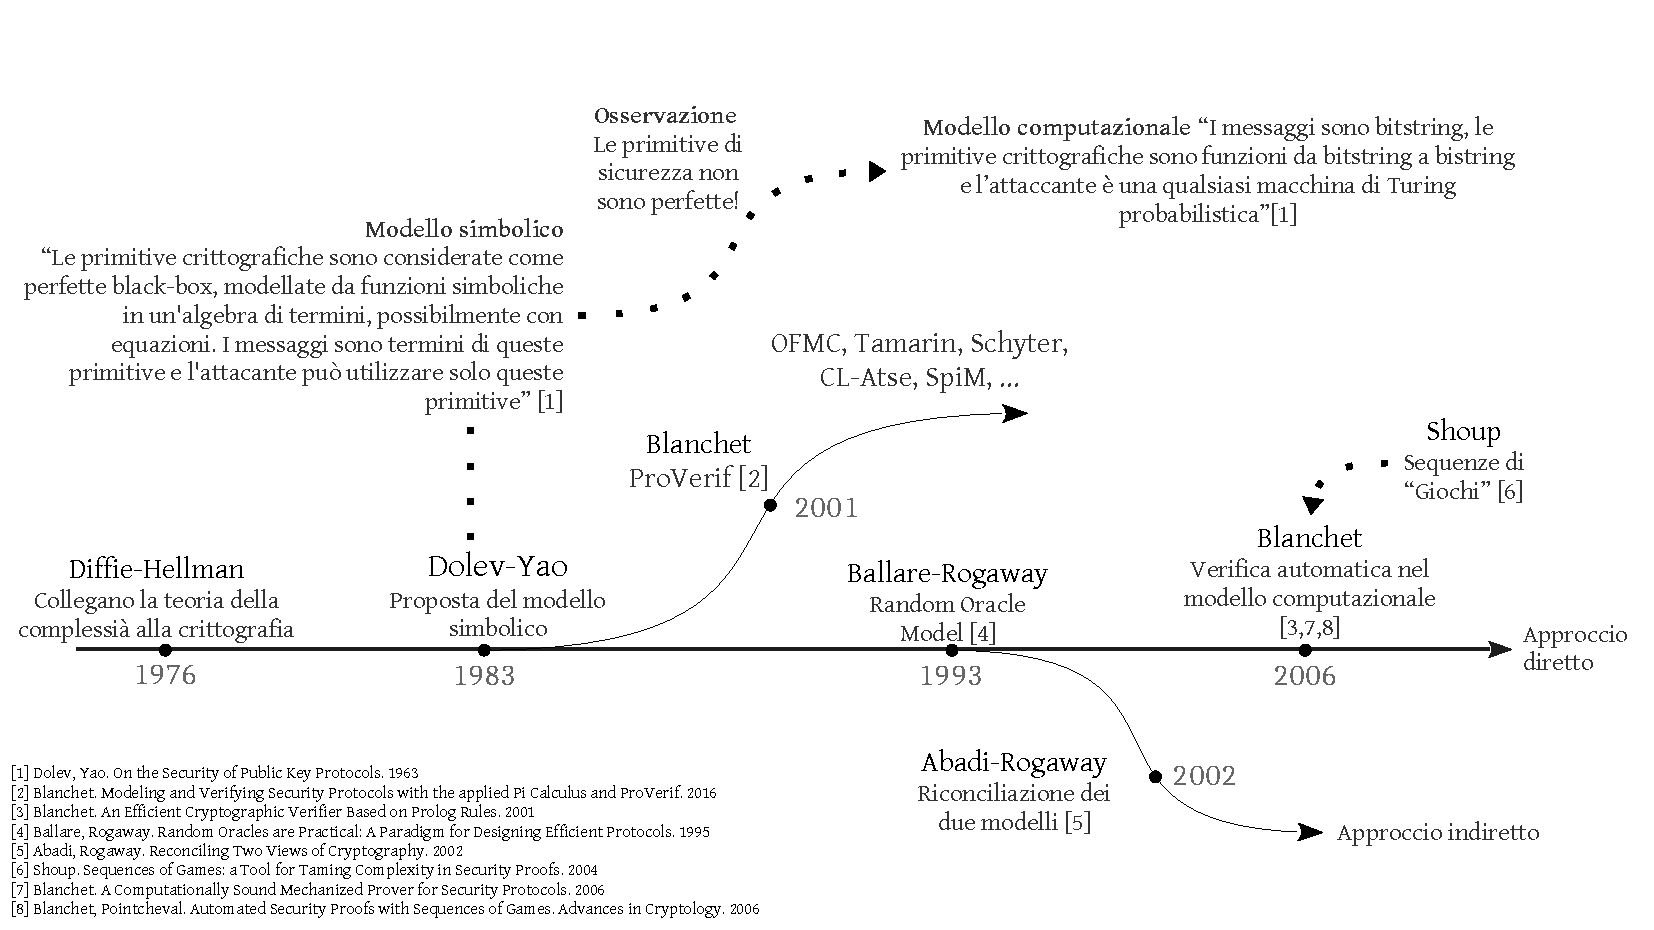
\includegraphics[width=\textwidth]{../img/evolution.pdf}}
    \caption{Evoluzione della ricerca negli anni}
    \label{fig:st} 
\end{figure}
\newpage

\newpage
\section{Tool per la verifica di protocolli basati sul modello simbolico}
\label{sez:tool}

Sviluppare un tool per la verifica automatica di protocolli basato sul modello simbolico resta comunque una sfida, questo perch\'e lo spazio di stati da esplorare è potenzialmente infinito per due motivi:
\begin{enumerate}
    \item la dimensione dello spazio dei messaggi non è definita in presenza di un attaccante attivo,
    \item il numero di sessioni del protocollo non è limitato.
\end{enumerate}
Una semplice soluzione a questo problema è quella di esplorare solo una parte dello spazio degli stati, limitando arbitrariamente sia la dimensione dello spazio dei messaggi che il numero di sessioni del protocollo.\\
Solo se il numero di sessioni è limitato, la verifica dei protocolli rimane decidibile: l'insicurezza del protocollo (esistenza di un attacco) è NP-completa con ipotesi ragionevoli sulle primitive crittografiche.\\
Nonostante questa indecidibilità, molte tecniche sono state progettate per verificare protocolli con un numero illimitato di sessioni, limitandosi a sottoclassi di protocolli, richiedendo l'interazione dell'utente, tollerando la non terminazione, o con sistemi incompleti (che possono rispondere ``Non lo so'').\\
In seguito verrano analizzati i tool per la verifica automatica dei protocolli basati sul modello simbolico ProVerif e VerifPal.\\

\subsection{ProVerif}\label{sub:pro}
Per la descrizione e l'analisi dei protocolli di sicurezza il tool ProVerif utilizza un linguaggio chiamato Applied Pi Calculus, un'estensione di Pi Calculus, il quale consente di dettagliare le azioni dei partecipanti al protocollo concentrando l'attenzione sulla loro comunicazione, più in generale consente di modellare processi concorrenti e la loro interazione.\\
A differenza del Pi Calculus vengono utilizzati termini al posto dei nomi per i messaggi.\\
Applied Pi Calculus \cite{AF16} è un linguaggio fortemente tipato che aggiunge a  Pi Calculus l'algebra utile a modellare le operazioni crittografiche utilizzate dai protocolli di sicurezza mediante una teoria equazionale (ad esempio l'operazione di modulo utilizzata nella generazione delle chiavi).\\
Inoltre consente di definire manualmente le primitive di sicurezza a differenza di un'altra estensione chiamata SPi Calculus \cite{AG97}, dove le primitive crittografiche come encryption e decryption sono implementate internamente.\\

\subsubsection*{Modellazione con ProVerif}

La modellazione di un protocollo in un file da dare in input a ProVerif può essere suddivisa in tre parti:
\begin{enumerate}
    \item dichiarazione formale del comportamento delle primitive crittografiche
    \item definizione di macroprocessi che consentono l'utilizzo di sotto-processi per semplificare lo sviluppo
    \item codifica del protocollo stesso come processo principale utilizzando le macro
\end{enumerate}

\subsubsection*{Dichiarazioni}
I processi sono composti da un insieme finito di tipi, nomi liberi e costruttori (funzioni simboliche) che
sono associati ad un insieme finito di decostruttori.\\ 
Il linguaggio è fortemente tipato e l'utente può definire dei nuovi tipi in questo modo: 
\begin{lstlisting}[language=app]
    type t . 
\end{lstlisting}
Tutti i nomi liberi devono essere dichiarati usando la sintassi: 
\begin{lstlisting}[language=app]
    free n : t .
\end{lstlisting} 
dove n è un nome e t il tipo.\\
La sintassi per dichiarare un canale è: 
\begin{lstlisting}[language=app]
    free c:channel.   
\end{lstlisting}
Tutte i nomi dichiarati con free sono conosciuti dall'attaccante, per fare in modo che non siano conosciuti dall'attaccante vanno dichiarati come privati utilizzando questa sintassi: 
\begin{lstlisting}[language=app]
    free n : t [ private ]. 
\end{lstlisting}
I costruttori (funzioni simboliche) sono usati per costruire termini di modellazione di primitive, usati dalla crittografia dei
protocolli, per esempio: funzioni di hash one-way, cifratura e firme digitali.\\
I costruttori si definiscono con:
\begin{lstlisting}[language=app, mathescape]
    fun $f(t_1,\dots, t_n )$ : t . 
\end{lstlisting} 
dove $f$ è un costruttore di arietà $n$, t è il tipo dell'oggetto di output e $t_1,\dots, t_n $ sono i tipi degli argomenti di input.\\
Anche i costruttori sono conosciuti dall'attaccante a meno della dichiarazione utilizzando [private].\\
I decostruttori vengono utilizzati per manipolare i termini formati dai costruttori e catturano le relazioni tra le primitive crittografiche, si modellano usando regole di riscrittura della forma:
\begin{lstlisting}[language=app, mathescape, breaklines= true]
    reduc forall $x_{1,1} : t_{1,1},\dots, x_{1,n_1}  : t_{1,n_1} ; 
    g(M_{1,1} , \dots , M_{1,k}) = M_{1,0} ;$
\end{lstlisting} 
dove $g$ è un decostruttore di arietà $k$, i termini $M_{1,1} , \dots , M_{1,k}, M_{1,0}$ sono costruiti dall'applicazione del costruttore alle variabili $x_{1,1},\dots, x_{1,n_1}$ di tipo $t_{1,1},\dots,t_{1,n_1}$ rispettivamente ed il tipo dell'output è $M_{1,0}$.\\
Analogamente ai costruttori, i decostruttori possono essere dichiarati privati con l'aggiunta di [private].\\
Vediamo come i costruttori e decostruttori vengono utilizzati per la definizione manuale delle primitive crittografiche:

\begin{lstlisting}[language=app]
    type key .
    fun senc(bitstring, key) : bitstring.
    reduc forall m: bitstring, k : key; 
        sdec(senc(m,k),k) = m.
\end{lstlisting}

\subsubsection*{Macro Processi}
Per semplificare lo sviluppo i sotto-processi vengono dichiarati utilizzando macro della forma: let $R(x_1:t_1,\dots,x_n:t_n) = P$., dove $R$ è il nome della macro, $P$ è il sotto-processo che si vuole definire e $x_1,\dots,x_n$ sono le variabili libere di $P$ di tipo $t_1,\dots,t_n$

\subsubsection*{Processi}

\begin{table}[h!]
    \begin{tabular}{ll}
        $M,N ::=$ & $termini$\\
        \quad$a, b, c, \dots , k, \dots , m, n, \dots , s$ & $nomi$\\
        \quad$x, y, z$ & $variabili$\\
        \quad$h(M_1, \dots , M_k)$ & $applicazione \: di \: costruttore/decostruttore$\\
        \quad $M=N$ & $uguaglianza \: tra \: termini$\\
        \quad $M<>N$ & $disuglianza \: tra \: termini$\\
        \quad $M\&\&N$ & $congiunzione$\\
        \quad $M||M$ & $disgiunzione$\\
        \quad not$M$ & $negazione$\\    
    \end{tabular}
    \caption{Grammatica di base}
    \label{tab:gb}
\end{table}

\begin{table}[h!]
    \begin{tabular}{ll}
        
        $P, Q::=$ & $processi$\\
        \quad$0$ & $processo \: vuoto$\\
        \quad$P|Q$ & $composizione \: parallela$\\
        \quad$!P$ & $replicazione$\\
        \quad new $n:t;P$ & $limitazione \: del \: nome$\\
        \quad$if \: M = N \: then \: P \: else \: Q$ & $condizione$\\
        \quad in$(M,x:t);P$ & $messaggio \: in \: input$\\
        \quad out$(M,N);P$ & $messaggio \: in \: output$\\
        \quad let $x=M \: in \: P \: else  \: Q$ & $valutazione \: del \: termine$\\
        \quad $R(M_1,\dots,M_k)$ & $utilizzo \: delle \: macro$\\       
    \end{tabular}
    \caption{Grammatica dei processi}
    \label{tab:gp}
\end{table}

\noindent Nella Tabella \ref{tab:gb} è descritta la grammatica di base dove i termini $M,N$ consistono in nomi $a, b, c, k, m, n, s$, variabili $x,y,z$, tuple ($M_1,\dots, M_l$) dove l è l'arietà della tupla, funzioni simboliche (costruttori/decostruttori) indicati con $h(M_1, \dots , M_k)$ dove k è l'arietà di h e gli argomenti $M_1,...,M_k$ sono del tipo richiesto.\\
Le altre funzioni utilizzano la notazione infissa e lavorano con l'algebra booleana.\\
Nella Tabella \ref{tab:gp} è descritta la grammatica dei processi dove il processo vuoto 0 non fa nulla, $P|Q$ è la composizione parallela di $P$ e $Q$, la replicazione $!P$ si comporta come un numero infinito di copie di $P$ in esecuzione in parallelo.\\ 
new $n:t;P$ lega il nome $n$ del tipo $t$ a $P$.\\
Il costrutto condizionale $if \: M = N \: then \: P \: else \: Q$ è standard e $M=N$ rappresenta l'uguaglianza, non l'identità.\\
Il processo in$(M,x:t);P$ indica che il processo $P$ è in attesa di un messaggio $x$ di tipo $t$ dal canale $M$ e poi prosegue la sua esecuzione.\\
Il processo out$(M,N);P$ indica che il processo $P$ è pronto per inviare $N$ nel canale $M$ e proseguire con la sua esecuzione.\\
Per evitare ambiguità durante l'esecuzione dei processi è consigliato utilizzare le parentesi per ordinarli.\\

\subsubsection*{Proprietà di sicurezza}
Per verificare la segretezza di un termine $M$ in un modello è sufficiente inserire la seguente query prima del processo principale:
\begin{lstlisting}[language=app]
    query attacker(M) .
\end{lstlisting} 
dove M è un nome di solito dichiarato privato, se così non fosse l'attaccante ne sarebbe banalmente a conoscenza.\\
Per verificare la proprietà di autenticazione è necessario annotare i processi con degli eventi in alcuni stati importanti, che non influiscono sul comportamento del protocollo.\\
Gli eventi verranno utilizzati per chiedere al tool se un determinato evento ha avuto luogo prima di un altro.\\
La sintassi per una richiesta di autenticazione è la seguente:
\begin{lstlisting}[language=app, mathescape]
    query $x_1:t_1 , \dots , x_n:t_n;$ 
    event $(e_1(M_1 ,\dots, M_j)) == >$ event $(e_0(N_1,\dots,N_k))$ .
\end{lstlisting} 
Ipotizzando che l'evento $e_0$ sia l'accettazione di un determinato client da parte di un server e l'evento $e_1$ sia l'invio di un messaggio dal client al server, con questo tipo di query ci chiediamo se il messaggio destinato al server è effettivamente stato inviato dal client corretto, nel caso in cui l'evento $e_0$ si sia effettivamente verificato prima dell'evento $e_1$, possiamo dire con certezza che il client è autenticato.\\
\noindent Ecco un esempio di come viene modellato in Applied Pi Calculus l'invio di un messaggio dall'agente A all'agente B e l'attaccante che prova ad intercettarlo:
\lstinputlisting[language=app, label={lst:hw}]{../code/hw.pv}


\subsection{VerifPal}
Tra i vari tool basati sul modello simbolico in grado di effettuare l'analisi formale dei protocolli di sicurezza, attualmente, il più utilizzato è ProVerif, purtroppo questo tool richiede all'utilizzatore di conoscere la sintassi del linguaggio Applied Pi Calculus, la quale è poco intuitiva, di conoscere il funzionamento delle clausole Horn create implicitamente dal tool e delle clausole Horn che devono essere esplicitate per modellare in maniera corretta lo scenario in cui verificare il protocollo.\\
Per questi motivi è stato sviluppato un nuovo tool chiamato VerifPal.\\
L'obiettivo di VerifPal è quello di descrivere protocolli con un linguaggio molto simile a come i protocolli potrebbero essere descritti in una conversazione informale.\\
Per fare ciò, pur basandosi internamente su costruzione e decostruzione di termini astratti simili a ProVerif, fa si che l'utente debba solo definire gli agenti partecipanti al protocollo che hanno stati indipendenti, conoscono determinati valori ed eseguono operazioni con le primitive crittografiche.\\
Le primitive crittografiche sono già definite e devono essere solo richiamate, in questo modo si evita che l'utente possa implementarle in maniera errata.\\
VerifPal \`e nato con lo scopo di creare un tool utilizzabile nell'ingegneria, per questo si presta ad essere utilizzato per il raggiungimento dell'obiettivo principale di questo documento, ovvero quello di utilizzare la modellazione UML per avvicinare la verifica di protocolli all'ingegneria di sistemi.  

\subsection*{Modellazione con VerifPal}
Quando si scrive il codice per la verifica formale di protocolli da analizzare con il tool VerifPal, la prima cosa da fare è scegliere se l'attaccante è di tipo attivo o di tipo passivo.\\
L'attaccante di tipo attivo viene comunemente chiamato attaccante di tipo Dolev-Yao (Sezione \ref{sec:dy}), mentre l'attaccante di tipo passivo è semplicemente un ascoltatore in grado di vedere i pacchetti che transitano sulla rete.\\
La seconda cosa da fare è inizializzare gli agenti che partecipano al protocollo, chiamati \texttt{principal}\footnote{questo tipo di font verrà applicato a tutte le keyword utilizzate da VerifPal}, all'interno della definizione dei principal possono essere definite delle costanti.\\ 
Queste costanti possono essere conoscenze pregresse del principal, per fare questo vengono inizializzate con la parola chiave \texttt{knows}, oppure possono essere delle costanti con dei valori generati al momento, in questo caso si utilizza la parola chiave \texttt{generates}.\\
Inoltre, le costanti possono essere definite pubbliche o private, nel caso in cui la costante sia definita pubblica anche l'attaccante ne è a conoscenza.\\
Per quanto detto sopra, per evitare errori da parte dell'utente, le variabili hanno uno scope globale, di conseguenza non possono esistere due costanti con lo stesso nome, a meno che non vengano definite come \texttt{private} e non possono essere riassegnate ad altri valori.\\
Una volta inizializzati i principal si passa alla modellazione del protocollo vero e proprio, con lo scambio dei messaggi e le varie operazioni fatte dai principal.\\
Per inviare un messaggio basta semplicemente indicare mittente, destinatario e contenuto del messaggio in questo modo: 
\begin{lstlisting}[mathescape]
    A$\rightarrow$B: m 
\end{lstlisting}
 Inoltre è possibile forzare il fatto che l'attaccante attivo non possa modificare il messaggio m semplicemente inserendolo tra $[$ $]$, l'utilizzo di questa tecnica di guardia è sconsigliato, in quanto potrebbe alterare il risultato della verifica, se non utilizzata correttamente.\\
Come detto sopra VerifPal ci viene incontro definendo le seguenti primitive (le quali corrispondono anche alle primitive del modello Dolev-Yao): 
\begin{itemize}
    \item \textbf{\texttt{CONCAT}}(a,b...) : c $\rightarrow$ concatena due o più valori in uno
    \item \textbf{\texttt{SPLIT}}(\textbf{\texttt{CONCAT}}(a,b...)) : a,b. $\rightarrow$ separa una concatenazione negli elementi che la compongono
    \item \textbf{\texttt{ENC}}(key,paintext) : ciphertext $\rightarrow$ codifica nella crittografia a chiave simmetrica
    \item \textbf{\texttt{DEC}}(key, \textbf{\texttt{ENC}}(key,paintext)): plaintext $\rightarrow$ decodifica nella crittografia a chiave simmetrica
    \item \textbf{\texttt{PKE\_ENC}}($G^{key}$, plaintext) : ciphertext $\rightarrow$ codifica nella crittografia a chiave asimmetrica
    \item \textbf{\texttt{PKE\_DEC}}(key, \textbf{\texttt{PKE\_ENC}}($G^{key}$, plaintext)) : plaintext $\rightarrow$ decodifica nella crittografia a chiave asimmetrica
    \item \textbf{\texttt{SIGN}}(key, message) : signature $\rightarrow$ firma un messaggio
    \item \textbf{\texttt{SIGNVERIF}}($G^{key}$, message, \textbf{\texttt{SIGN}}(key, message)) : message $\rightarrow$ verifica della firma
\end{itemize}

\noindent Oltre a queste primitive VerifPal fornisce altre primitive utili per effettuare l'hash dei messaggi.\\
Il modello del protocollo si conclude con un blocco chiamato \texttt{queries}, dove sono contenute le domande alle quali vorremmo che VerifPal ci desse le risposte come risultato dell'analisi del modello.\\
Nel blocco di queries possiamo fare delle domande su confidenzialità, autenticazione, freshness dei messaggi utilizzando rispettivamente i comandi \texttt{confidentiality?}, \texttt{authentication?} e \texttt{freshness?}.\\
Inoltre nel caso in cui si volesse modellare uno scenario in cui l'attaccante riesce ad ottenere una costante dichiarata come privata in qualche modo, basta utilizzare la parola chiave \texttt{leaks} seguita dal nome della variabile.\\
Qui è proposto lo stesso scenario modellato nella Sezione \ref{lst:hw} con ProVerif:
\lstinputlisting[language=vp]{../code/test.vp}



\section{Conclusioni}
Abbiamo visto come la verifica formale dei protocolli di sicurezza sia un'operazione importante, da effettuare prima di utilizzare un protocollo all'interno di un'applicazione o di un software, per garantire la sicurezza dei dati e delle informazioni.\\
Inoltre abbiamo visto come allo stato dell'arte esistano il modello computazionale e il modello simbolico per la verifica formale automatica dei protocolli, ma solo il modello simbolico, il quale utilizza l'attaccante del modello Dolev-Yao, è abbastanza ``maturo'' per essere effettivamente utilizzato.\\ 
In questo documento è stato presentato un nuovo modo, intuitivo e agile, per modellare i protocolli mediante diagrammi UML, che può essere utilizzato dai progettisti ed è stata fatta un'analisi su limiti e capacità delle tecniche di modellazione attuali. \\
\`E stato presentato il software sviluppato appositamente per trasformare i protocolli modellati mediante diagrammi UML in un file utilizzabile come input per il tool di verifica automatica VerifPal.\\
I protocolli analizzati con VerifPal ci hanno consentito di analizzare limiti e capacità di questo tool di verifica automatica e di verificarne la bontà dei risultati di analisi.\\
Un obiettivo futuro può essere quello di utilizzare i software open source Modelio e VerifPal insieme al tool di conversione  presentato, per creare un unico software open source in grado di consentire ai progettisti di modellare i protocolli tramite diagrammi UML ed avere immediatamente garanzie sulla sicurezza dei protocolli.

\newpage
%\appendix
%\subsection{Modellazione di protocolli con UML}
%\fixnote{mr}{non possiamo avere cos\`i tanti esempi senza spiegazione. O li raccontiamo o li togliamo. Se ``spaccano'' troppo il testo possiamo spostarli in appendice. Inoltre le immagini sono difficili da leggere perch\'e ci sono troppi a-capo nei blocchi. Inoltre le varie immagini sono zoomate diversamente, io renderei pi\`u omogeneo.}
\subsubsection*{Needham Schroeder Symmetric Key}
In questa sezione vedremo come è possibile modellare attraverso i diagrammi object diagram dello standard UML il protocollo di sicurezza a chiave simmetrica proposto da Needham e Schroeder:
\begin{lstlisting}[mathescape]
    1. $A \rightarrow S : A, B, N_a$
    2. $S \rightarrow A : \{N_a, K_{ab}, B, \{K_{ab}, A\}_{K_{bs}}\}_{K_{as}}$
    3. $A \rightarrow B : \{K_{ab}, A\}_{K_{bs}}$
    4. $B \rightarrow A : \{N_b\}_{K_{as}}$
    5. $A \rightarrow B : \{N_b-1\}_{K_{as}}$
\end{lstlisting} 

\noindent Nelle Figure seguenti avremo i seguenti partecipanti al protocollo: l'agente Initiator che vuole iniziare la comunicazione con l'agente Recipient e richiede la password per la comunicazione al server S.\\
Inoltre la chiave simmetrica viene rappresentata in questo modo SK(a,b), dove a e b indicano l'identità degli agenti proprietari della chiave.\\

\begin{figure}[h!] 
    \centering 
    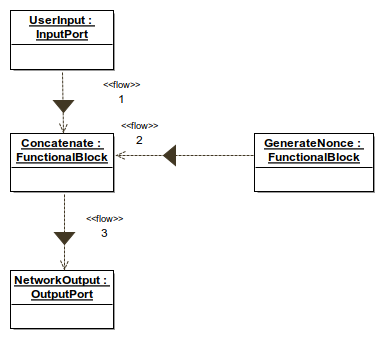
\includegraphics[scale=0.6]{img/NSSK/First_message(toServer)_Object diagram.png} 
    %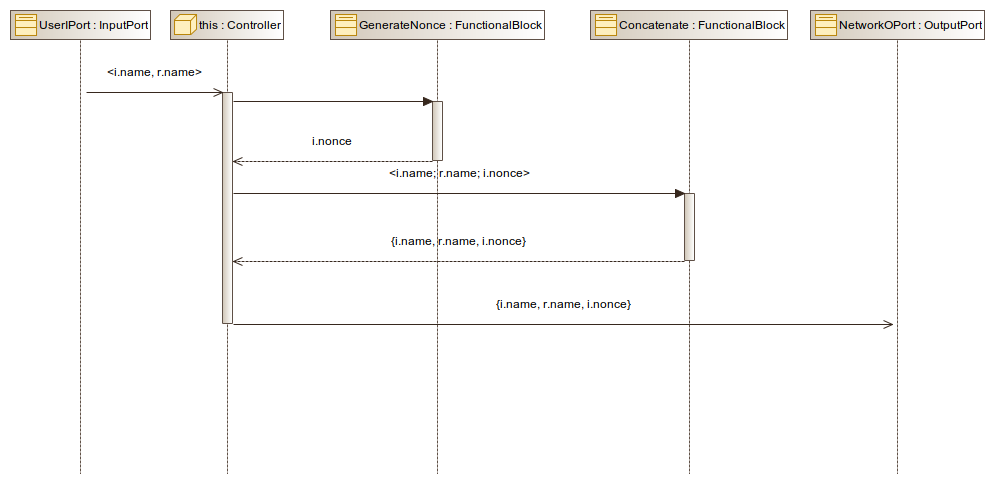
\includegraphics[width=\textwidth]{img/NSSK/Sequencediagram/First_Message(toServer).png} 
    \begin{lstlisting}[frame=single, mathescape, basicstyle=\footnotesize]
        1. $<i.name, r.name>$
        2. $<i.nonce>$
        3. $<i.name, r.name, i.nonce>$
    \end{lstlisting}
    \caption{$A \rightarrow B : A, B, N_a$} 
\end{figure}
\noindent Nell'oggetto UserInput il sistema che andrà ad implementare il protocollo riceve il nome ($r.name$) dell'agente Recipient, l'oggetto GenerateNonce genera un nuovo Nonce e l'oggetto Concatenate prepare il pacchetto, da mandare al server S attaverso l'oggetto NetworkOPort, composto da $i.name, r.name, i.nonce$, ovvero dai nomi dei partecipanti al protocollo e il nonce per assicurarsi che la comunicazione sia fresh.
\newpage
\begin{figure}[h!] 
    \centering 
    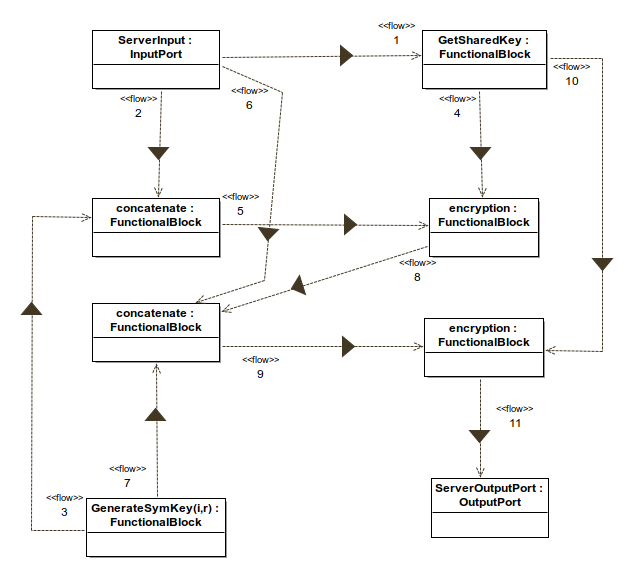
\includegraphics[scale=0.5]{img/NSSK/Second_Message(fromServer).png} 
    %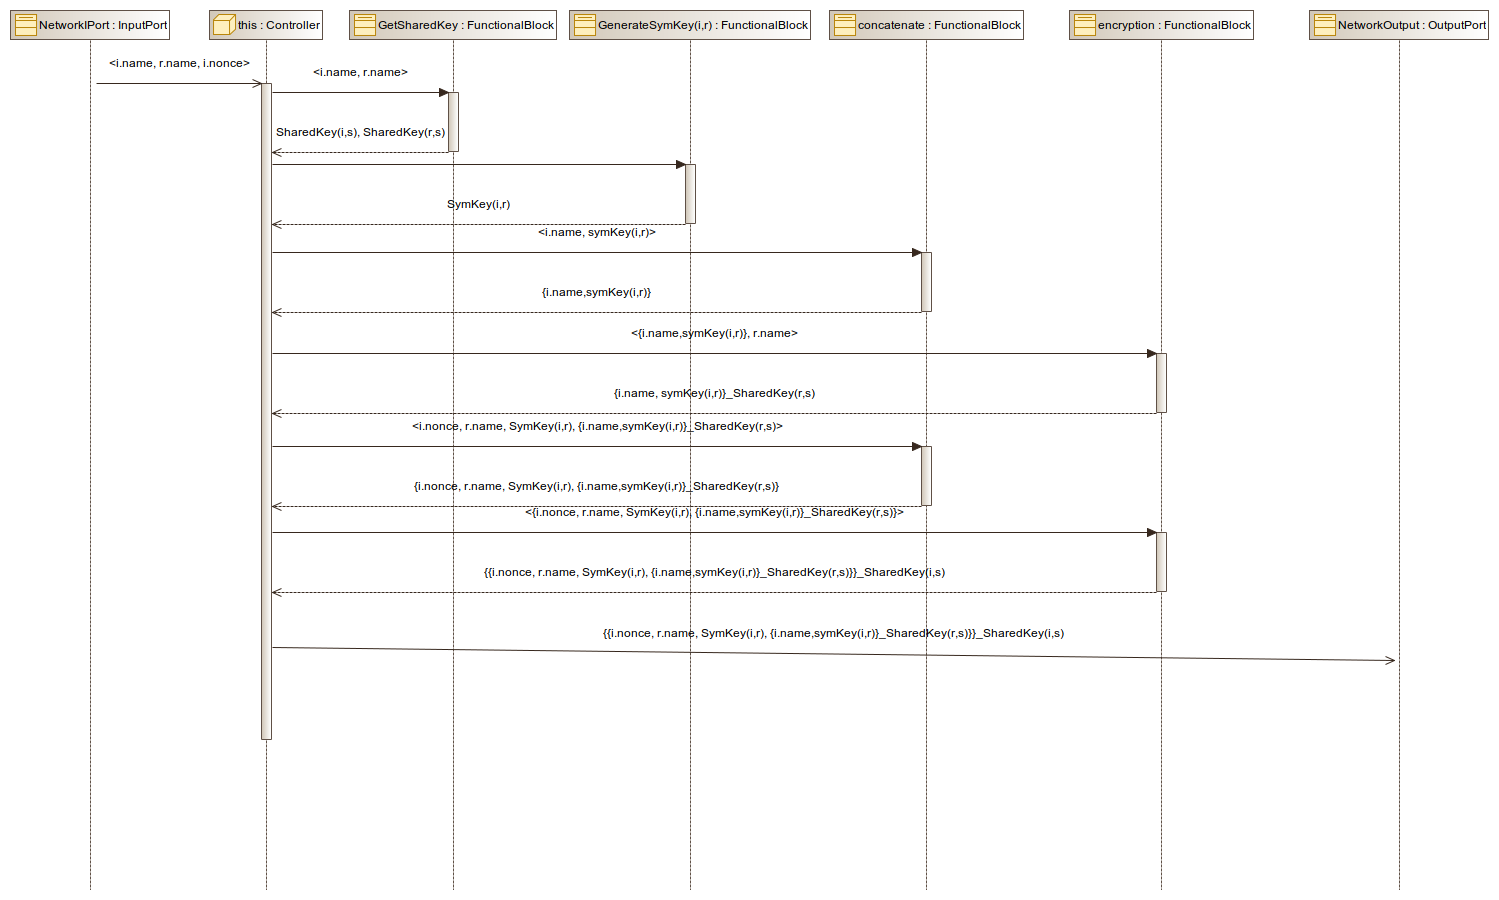
\includegraphics[width=\textwidth]{img/NSSK/Sequencediagram/Second_Message(fromServer).png} 
    \begin{lstlisting}[frame=single, mathescape, basicstyle=\footnotesize]
        1. $<i.name,r.name>$
        2. $<i.name>$
        3. $<SK(i,r)>$
        4. $<SK(s,r)>$
        5. $<i.name, SK(i,r)>$
        6. $<r.name, i.nonce>$
        7. $<SK(i,r)>$
        8. $<\{i.name; SK(i,r)\}\_SK(r,s)>$
        9. $<i.nonce, r.name, SK(i,r), \{i.name,SymKey(i,r)\}\_SK(r,s)\}>$
        10. $<SK(s,r)>$
        11. $<\{i.nonce, r.name, SK(i,r), \{i.name,SK(i,r)\}\_SK(rs)\}\}\_SK(i,s)>$
    \end{lstlisting}
    \caption{$S \rightarrow A : \{N_a, K_{ab}, B, \{K_{ab}, A\}_{K_{bs}}\}_{K_{as}}$} 
\end{figure}
\noindent Una volta ricevuto il pacchetto, il server S provvede alla generazione della chiave simmetrica (SK(i,r)) per la comunicazione tra Initiator e Recipient utilizzando l'oggetto GenerateSymKey(i,r), passando a quest'ultimo i nomi $i.name, r.name$ dei partecipanti.\\ 
A questo punto, fornendo sempre come input i nomi dei partecipanti all'oggetto GetSharedKey, ottiene le chiavi simmetriche precedentemente condivise tra lui e ogni agente partecipante (SK(i,s) e SK(r,s)).\\ 
La chiave SK(r,s) verrà utilizzata dall'oggetto encryption dopo aver preparato con l'oggetto Concatenate il pacchetto per l'agente Recipient, questo pacchetto a sua volta verrà inserito da un altro oggetto Concatenate nel pacchetto per l'agente Initiator e il tutto verrà cifrato da un'altro oggetto encryption con la chiave SK(i,s). Il pacchetto risultante da queste operazioni verrà spedito all'agente Initiator attraverso l'oggetto ServerOutputPort.\\

\begin{figure}[h!] 
    \centering 
    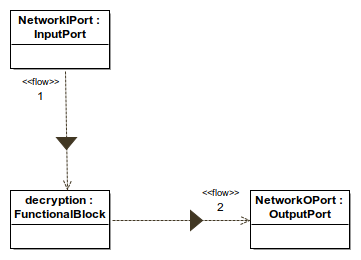
\includegraphics[scale=0.6]{img/NSSK/FirstMessage.png} 
    %\includegraphics[width=\textwidth]{img/NSSK/Sequencediagram/FirstMessage.png}
    \begin{lstlisting}[frame=single, mathescape, basicstyle=\footnotesize]
        1. $<\{i.nonce, r.name, SK(i,r), \{i.name,SK(i,r)\}\_SK(r,s)\}\_SK(i,s)>$
        2. $<\{i.name,SK(i,r)\}\_SK(r,s)>$
    \end{lstlisting}
    \caption{$A \rightarrow B : \{K_{ab}, A\}_{K_{bs}}$} 
\end{figure}
\noindent L'agente Initiator riceve il pacchetto attraverso l'oggetto NetworkIPort e utilizza l'oggetto di decryption con la chiave simmetrica SK(i,s) per estrarre il pacchetto da inoltrare all'agente Recipient attraverso l'oggetto NetworkOPort.\\
\begin{figure}[h!] 
    \centering 
    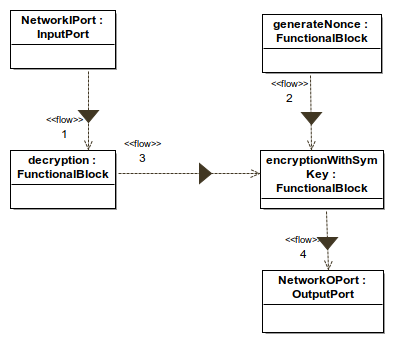
\includegraphics[scale=0.59]{img/NSSK/SecondMessage.png} 
    %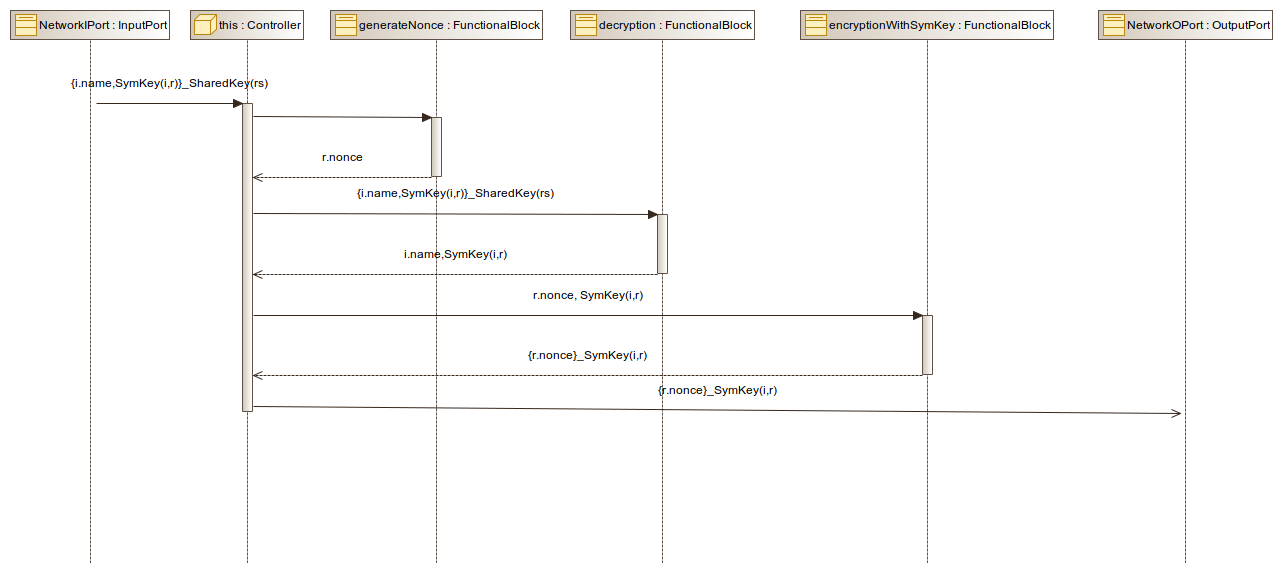
\includegraphics[width=\textwidth]{img/NSSK/Sequencediagram/SecondMessage.png} 
    \begin{lstlisting}[frame=single, mathescape, basicstyle=\footnotesize]
        1. $<\{i.name,SK(i,r)\}\_SK(r,s)>$
        2. $<r.nonce>$
        3. $<SK(i,s)>$
        4. $<\{r.nonce\}\_SK(i,r)>$
    \end{lstlisting}
    \caption{$B \rightarrow A : \{N_b\}_{K_{as}}$} 
\end{figure}
\newpage
\noindent L'agente Recipient riceve il pacchetto attraverso l'oggetto NetworkIPort, lo decifra con l'oggetto decryption utilizzando la chiave SK(r,s) ed estrae la chiave SK(i,r).\\ 
SK(i,r) verrà utilizzata dall'oggetto encryptionWithSymKey per cifrare un nuovo pacchetto contenente il Nonce generato dall'oggetto generateNonce.\\ 
Infine l'agente Recipient spedisce il pacchetto all'agente Initiator utilizzando l'oggetto NetworkOPort.\\
\begin{figure}[h!] 
    \centering 
    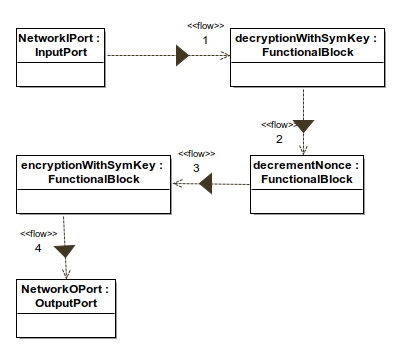
\includegraphics[scale=0.6]{img/NSSK/ThirdMessage.png} 
    %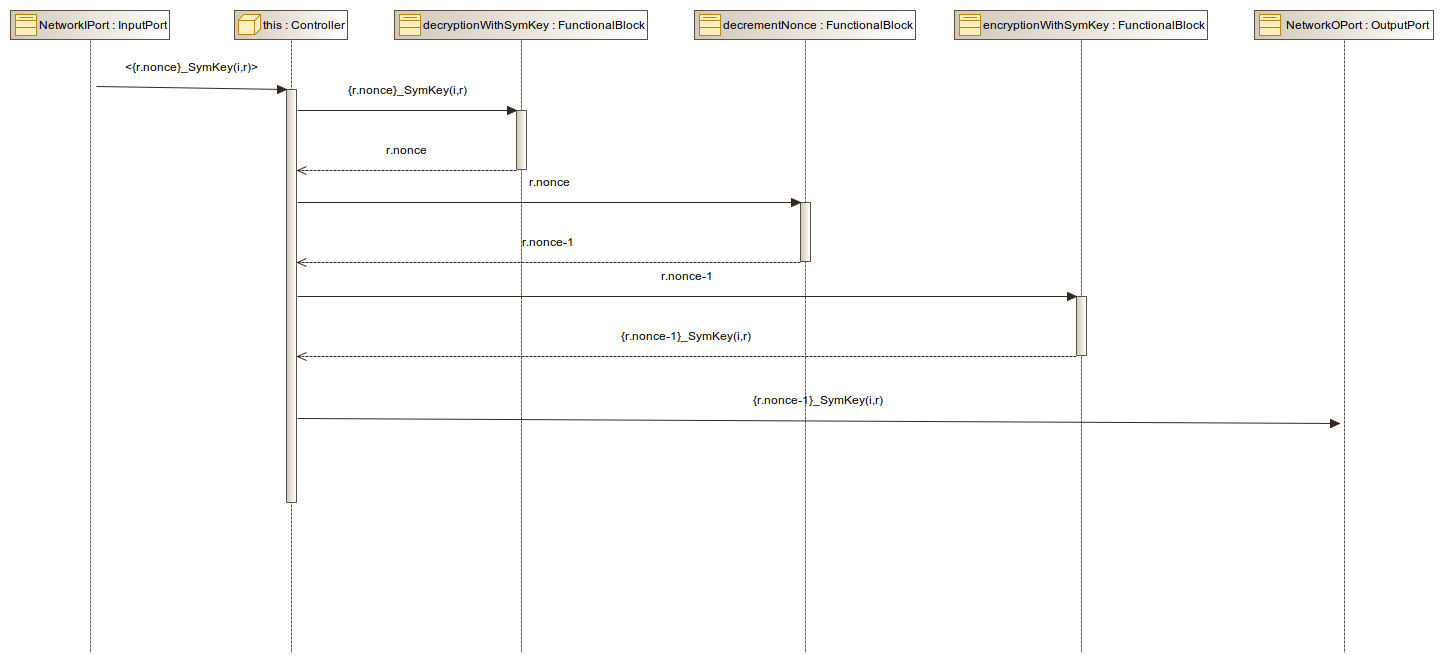
\includegraphics[width=\textwidth]{img/NSSK/Sequencediagram/ThirdMessage.png} 
    \begin{lstlisting}[frame=single, mathescape, basicstyle=\footnotesize]
        1. $<{r.nonce}\_SK(i,r)>$
        2. $<r.nonce>$
        3. $<r.nonce-1>$
        4. $<\{r.nonce-1\}\_SK(i,r)>$
    \end{lstlisting}
    \caption{$A \rightarrow B : \{N_b-1\}_{K_{as}}$} 
\end{figure}\\
\noindent Nell'ultima fase del protocollo, l'agente Initiator riceve dall'oggetto NetworkIPort il pacchetto contenente il Nonce, lo decifra con l'oggetto decryptionWithSymKey utilizzando la chiave SK(i,r), utilizza l'oggetto decrementNonce per sottrarre 1 al Nonce inviato dall'agente Recipient e cifra il risultato con l'oggetto encryptionWithSymKey utilizzando la chiave SK(i,r).\\
Il pacchetto risultante viene spedito all'agente Recipient attraverso l'oggetto NetworkOPort.\\

\newpage
\subsubsection*{Address Resolution Protocol}
Lo scopo del protocollo ARP descritto in \cite{RFC0826} e in \cite{RFC5227} è quello di eseguire una mappatura tra indirizzo IP e indirizzo MAC di una macchina all'interno di una rete locale Ethernet.\\
La notazione seguente utilizzata nei pacchetti è ripresa da \cite{RFC0826}:
\begin{lstlisting}
    ar$hrd: Hardware address space 
    ar$pro: Protocol address space
    ar$hln: byte length of each hardware address
    ar$pln: byte length of each protocol address
    ar$op:  opcode (request | reply)
    ar$sha: Hardware address of sender 
    ar$spa: Protocol address of sender 
    ar$tha: Hardware address of target
    ar$tpa: Protocol address of target
\end{lstlisting}
In Figura \ref*{fig:ARP} vediamo come si modella il protocollo ARP.\\
Una macchina, appena connessa alla rete o accesa, si mette subito in ascolto con l'oggetto ANNUNCE\_AWAIT e, allo stesso tempo, utilizza gli oggetti getIPAddress per generare un indirizzo IP sul quale essere contattata, getProtocolType e getMACAddress  per ricavare informazioni sul tipo di protocollo ethernet da utilizzare e l'indirizzo MAC della sua scheda di rete.\\
A questo punto utilizza queste informazioni per creare attraverso l'oggetto createProbePackage un pacchetto da inviare in broadcast a tutte le macchine della rete.\\
Successivamente attende un tempo predefinito attraverso l'oggetto PROBE\_WAIT, prima di spedire il pacchetto attraverso l'oggetto EthernetOUT e ritornare nello stato di ANNUNCE\_WAIT.\\
Se nell'arco di un tempo predefinito non arriva nessun pacchetto dall'oggetto EthernetIN, procede con la conferma dell'indirizzo IP attraverso la creazione di un nuovo pacchetto con l'oggetto createAnnuncePackage, il quale verra sempre spedito in broadcast attraverso l'oggetto EthernetOUT.\\
Se invece riceve un pacchetto dall'oggetto EthernetIN, ricomincia generando un nuovo indirizzo IP.\\
\newpage
\begin{figure}[h!] 
    \centering 
    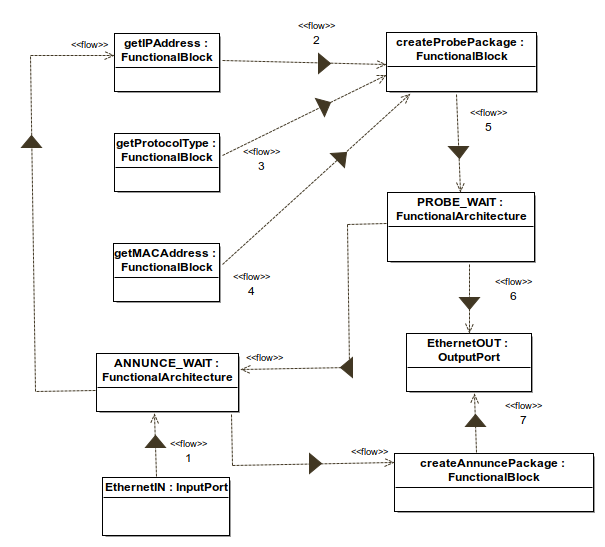
\includegraphics[scale=0.6]{img/ARP/ARP.png} 
    \begin{lstlisting}[frame=single, mathescape, basicstyle=\footnotesize]
1. $<\{as\$hrd, ar\$pro, ar\$hln, ar\$pln, reply, ar\$sha, ar\$spa, ar\$tha, ar\$tpa\}>$
2. $<ip>$
3. $<ar\$spa>$
4. $<ar\$sha>$
5. $<\{as\$hrd, ar\$pro, ar\$hln, ar\$pln, request, ar\$sha, 0.0.0.0, 00:00:00:00:00:00, ip\}>$
6. $<\{as\$hrd, ar\$pro, ar\$hln, ar\$pln, request, ar\$sha, 0.0.0.0, 00:00:00:00:00:00, ip\}>$
7. $<\{as\$hrd, ar\$pro, ar\$hln, ar\$pln, request, ar\$sha, ip, 00:00:00:00:00:00, ip\}>$
    \end{lstlisting}
    \caption{Modellazione del protocollo ARP} 
    \label{fig:ARP}
\end{figure}
\newpage
\begin{figure}[h!] 
    \centering 
    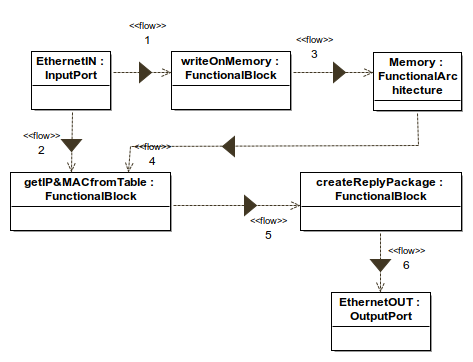
\includegraphics[scale=0.6]{img/ARP/ARP_Reply_Object_diagram.png} 
\begin{lstlisting}[frame=single, mathescape, basicstyle=\footnotesize]
1. $<\{as\$hrd, ar\$pro, ar\$hln, ar\$pln, request, ar\$sha, ip, 00:00:00:00:00:00, ip\}>$
2. $<\{as\$hrd, ar\$pro, ar\$hln, ar\$pln, request, ar\$sha, 0.0.0.0, 00:00:00:00:00:00, ip\}>$
3. $<ar\$sha, ip>$
4. $<ar\$tha, ar\$tpa>$
5. $<ar\$tha, ar\$tpa>$
6. $<\{as\$hrd, ar\$pro, ar\$hln, ar\$pln, reply, ar\$sha, ar\$spa, ar\$tha, ar\$tpa\}>$
\end{lstlisting}
    \caption{Modellazione del blocco di ARP Reply} 
\end{figure}
\noindent Nel caso in cui una macchina della rete riceva un pacchetto dall'oggetto EthernetIN, la prima cosa che fa è verificare se si tratta di un pacchetto di probe oppure di un pacchetto di annunce.\\
Nel primo caso va a verificare con l'oggetto Memory se nell'ARP cache è già presente quell'indirizzo IP, assegnato ad un indirizzo MAC, che non corrisponde a quello del sender del pacchetto.\\ 
Se vi è una corrispondenza tra l'indirizzo ip del sender del pacchetto ed uno già presente nell'ARP cache, allora l'oggetto getIP\&MACFromTable riceve in input le informazioni dalla ARP cache per generare un nuovo pacchetto attraverso l'oggetto createReplyPackage, con il quale rispondere in unicast al sender attraverso l'oggetto EthernetOut, altrimenti non fa nulla.\\
Nel caso in cui si tratti di un pacchetto di annunce allora l'oggetto writeOnMemory si occuperà di salvare nella ARP cache la mappatura tra l'indirizzo IP e MAC del sender.\\
\newpage
\clearpage
\subsubsection*{RSA}
Nel 1978 in \cite{RSA78} Rivest, Shamir e Adleman hanno proposto un crittosistema per la cifratura e la firma dei messaggi basato sulla crittografia asimmetrica.\\
Come vedremo nelle Figure successive il crittosistema si basa su tre funzioni principali: funzione di generazione delle chiavi, funzione di encryption e funzione di decryption.\\
Nella modellazione UML ogni oggetto rappresenta le funzioni matematiche utilizzate dalle tre funzioni.\\ 
L'oggetto Memory viene utilizzato dalla funzione di generazione delle chiavi per salvare le informazioni riguardo la chiave pubblica e la chiave privata necessarie alle funzioni di encryption e decryption.\\  
\begin{figure}[h!] 
    \centering 
    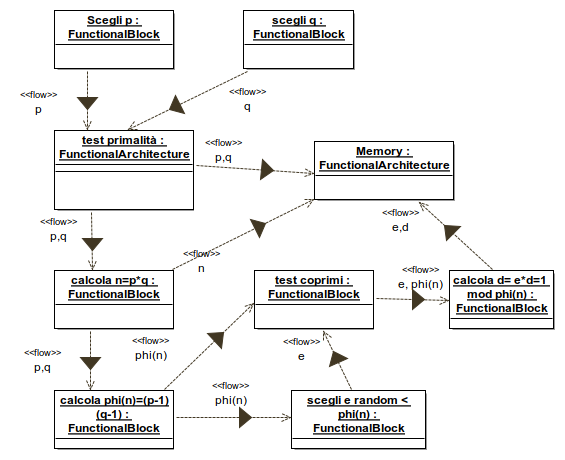
\includegraphics[scale=0.6]{img/RSA/Key_Generation_Object_diagram.png} 
    \caption{Generazione delle chiavi} 
\end{figure}
\begin{figure}[h!] 
    \centering 
    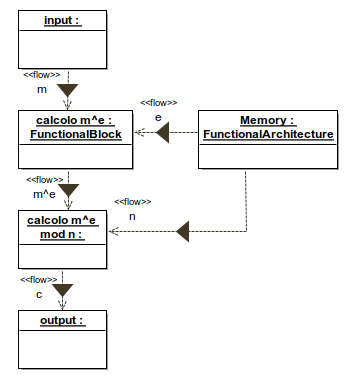
\includegraphics[scale=0.6]{img/RSA/Encryption_Object_diagram.png} 
    \caption{Funzione di encryption} 
\end{figure}
\newpage
\begin{figure}[h!] 
    \centering 
    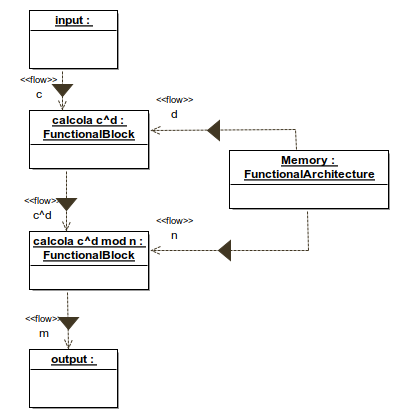
\includegraphics[scale=0.6]{img/RSA/Decryption_Object_diagram.png} 
    \caption{Funzione di decryption} 
\end{figure}
\newpage



    





%\bibliographystyle{natdin}
%\bibliographystyle{apalike}
%\bibliography{reference.bib}
\newpage
\clearpage
\printbibliography



\end{document}

